\documentclass[twoside]{book}

% Packages required by doxygen
\usepackage{calc}
\usepackage{doxygen}
\usepackage{graphicx}
\usepackage[utf8]{inputenc}
\usepackage{makeidx}
\usepackage{multicol}
\usepackage{multirow}
\usepackage{textcomp}
\usepackage[table]{xcolor}

% Font selection
\usepackage[T1]{fontenc}
\usepackage{mathptmx}
\usepackage[scaled=.90]{helvet}
\usepackage{courier}
\usepackage{amssymb}
\usepackage{sectsty}
\renewcommand{\familydefault}{\sfdefault}
\allsectionsfont{%
  \fontseries{bc}\selectfont%
  \color{darkgray}%
}
\renewcommand{\DoxyLabelFont}{%
  \fontseries{bc}\selectfont%
  \color{darkgray}%
}

% Page & text layout
\usepackage{geometry}
\geometry{%
  a4paper,%
  top=2.5cm,%
  bottom=2.5cm,%
  left=2.5cm,%
  right=2.5cm%
}
\tolerance=750
\hfuzz=15pt
\hbadness=750
\setlength{\emergencystretch}{15pt}
\setlength{\parindent}{0cm}
\setlength{\parskip}{0.2cm}
\makeatletter
\renewcommand{\paragraph}{%
  \@startsection{paragraph}{4}{0ex}{-1.0ex}{1.0ex}{%
    \normalfont\normalsize\bfseries\SS@parafont%
  }%
}
\renewcommand{\subparagraph}{%
  \@startsection{subparagraph}{5}{0ex}{-1.0ex}{1.0ex}{%
    \normalfont\normalsize\bfseries\SS@subparafont%
  }%
}
\makeatother

% Headers & footers
\usepackage{fancyhdr}
\pagestyle{fancyplain}
\fancyhead[LE]{\fancyplain{}{\bfseries\thepage}}
\fancyhead[CE]{\fancyplain{}{}}
\fancyhead[RE]{\fancyplain{}{\bfseries\leftmark}}
\fancyhead[LO]{\fancyplain{}{\bfseries\rightmark}}
\fancyhead[CO]{\fancyplain{}{}}
\fancyhead[RO]{\fancyplain{}{\bfseries\thepage}}
\fancyfoot[LE]{\fancyplain{}{}}
\fancyfoot[CE]{\fancyplain{}{}}
\fancyfoot[RE]{\fancyplain{}{\bfseries\scriptsize Generated on Thu Mar 27 2014 20:22:00 for SPH Water Simulation by Doxygen }}
\fancyfoot[LO]{\fancyplain{}{\bfseries\scriptsize Generated on Thu Mar 27 2014 20:22:00 for SPH Water Simulation by Doxygen }}
\fancyfoot[CO]{\fancyplain{}{}}
\fancyfoot[RO]{\fancyplain{}{}}
\renewcommand{\footrulewidth}{0.4pt}
\renewcommand{\chaptermark}[1]{%
  \markboth{#1}{}%
}
\renewcommand{\sectionmark}[1]{%
  \markright{\thesection\ #1}%
}

% Indices & bibliography
\usepackage{natbib}
\usepackage[titles]{tocloft}
\setcounter{tocdepth}{3}
\setcounter{secnumdepth}{5}
\makeindex

% Hyperlinks (required, but should be loaded last)
\usepackage{ifpdf}
\ifpdf
  \usepackage[pdftex,pagebackref=true]{hyperref}
\else
  \usepackage[ps2pdf,pagebackref=true]{hyperref}
\fi
\hypersetup{%
  colorlinks=true,%
  linkcolor=blue,%
  citecolor=blue,%
  unicode%
}

% Custom commands
\newcommand{\clearemptydoublepage}{%
  \newpage{\pagestyle{empty}\cleardoublepage}%
}


%===== C O N T E N T S =====

\begin{document}

% Titlepage & ToC
\hypersetup{pageanchor=false}
\pagenumbering{roman}
\begin{titlepage}
\vspace*{7cm}
\begin{center}%
{\Large S\-P\-H Water Simulation \\[1ex]\large 1.\-0 }\\
\vspace*{1cm}
{\large Generated by Doxygen 1.8.4}\\
\vspace*{0.5cm}
{\small Thu Mar 27 2014 20:22:00}\\
\end{center}
\end{titlepage}
\clearemptydoublepage
\tableofcontents
\clearemptydoublepage
\pagenumbering{arabic}
\hypersetup{pageanchor=true}

%--- Begin generated contents ---
\chapter{S\-P\-H Water Simulation by Declan Russll}
\label{index}\hypertarget{index}{}  This program should run pretty much out of the box, just rebuild all once you boot up the project and click run!\par
  Space -\/ play/pause our simulation \par
 1 -\/ toggle drawing of the mesh \par
 2 -\/ toggle drawing of the particles \par
 3 -\/ toggle between our mesh simulation and my brand new 2d simulation! \par
 Left click -\/ Rotate the scene \par
 Right click -\/ Pan the scene\par
 Ctrl + Left click -\/ Move the external force postion. You can click and drag with this\par
 +/-\/ -\/ increase and decrease the strength of the external force\par
 0/9 -\/ increase and decrease the radial influence of the external force. Note this force has linear falloff\par
 E -\/ toggle the force between pushing and sucking\par
 R -\/ restart the simulation\par
 Feel free to change the input mesh, just change the model\-Location in \hyperlink{classNGLScene_a63e57fc201b639e51c6eed6ec3b6b992}{N\-G\-L\-Scene\-::initialize()}\par
  Navier Stokes Equations\par
 The over all Navier stokes euquation goes as follows,\par
  This calculates the acceleration of a particle. Now although this may look quite complicated we can break it down into 3 main parts.\par
 \par
 The Density of the particle\par
  In the equation xi is the position of the particle that we wish to find the density for. So to find the density for this particle we sum together the mass of neighbouring particles j multiplied by weighting kernal W.\par
 What is a weighting kernal?\par
 The weighting kernal determins the influence each particle has one each other. For instance if 2 particle are very close, then the influence will be very high. Alternativly if the two particles are very far away from each other they will have very low or zero influence on each other.\par
 \par
 Calculateing the weighting kernal\par
  In this equation there are 2 variables.\par
 'r' This is the distance between the particle we are calculating density for and the neighbouring particle we are sampling.\par
 'h' this is our smoothing length. This ultimately determins the distance in which the particles continue to have infulence. You can see this from the limitations in our W default equation. If r $>$ h then we will return 0 and this particle will have no influence.

The Pressure gradient\par
  This is the pressure gradient, this indicates the direction of pressure and how dtring it is. If the pressure is negative then there is a sucking force, alternatively is positive then it is a pushing force. This equation is slightly more complicated that the previous but again if we split it up it becomes much easier to handle. We'll start with the part in the brackets. The p stands for pressure, pi is the pressure of the particle that we are calculating for and pj is the neighbouring particle that we are sampling. But how do we calculate the pressure you may ask?\par
  This euqation calculates the pressure per particle. Row (the p shaped letter) stands for density. Rowi is our current density and Row0 is the resting density of our particle. k is a gas constant which we can change depending on what fluid we are trying to imitate.\par
 Moving onto the next part of the pressure equation we have mj which is simply the mass of our neighbouring particle, multiplied by another weighting kernal. \par
 Calculating the pressure wighting kernal\par
  As you can see this weighting kernal is very similar to our density one. 'r' is still the distance between particles and 'h' is still our smoothing length. Notice the Wdefault, this means that we still have the same limitations that we did in our density kernal.\par
 The Viscosity Term\par
  The Viscosity in simple terms influences particles to flow in the same direction. If a large amount of particles are moving in one direction others should follow them.\par
 Lets break this equation down. Firstly we have meu, this represents our viscosity coeficitent, a scaler to our viscosity equation. This can be changed depending on what liquid we are trying to imitate. Next 'u', this is the velocity of a particle. (uj -\/ ui) is the vector from our currents particles velcity to our neighbours. 'm' we already know as mass and 'Row' we know as the density. Finally we have our third and final weighting kernal. \par
 Calculating the viscosity weighting kernal\par
  Just like before we have 'r' the distance between particles and 'h' our smoothing length. Once again we just pump in these values to calculate the influence weight of this particle.\par
 Any External Forces\par
  External forces in this simulation can be things such as gravity or wind. In my simulation I have used this to create a external force to interact with the fluid from mouse clicks.\par
 \par
  As you can see the Navier stokes equations calculate the acceleration of our particles. From this we can use the time step between updates to calcute our velcocity and our postion of our particles. The first itegrator I used was simple Euler euqations,  Here we have 2 equations, the first to calculate 'u' our velocity for a particle. This uses 'a' our calculated acceleration and delta(the d) t, which represents the change in time. The second equation calculates 'x' our postion in a similar way. Also though these euqations are acurate in real world physics, for our simulations they will create large errors due to the delay between updating each particle. So we must use another method.\par
   This is the Leap Frog integration method. It works by using future half step velocities to calculate a more accurate value for position. To calculate the actual velocity at a point in time from these half step velocies we must use a forth equation.  This uses our half back velocity and our half forward to calculate our final particle velocity. \par
  For this simulation, for us to achieve a respectable frame rate we are going to have to sacrifice some accuracy in our equations. The Navier Stokes equations in real life implementation need to sample every point in exsistance to find the true acceleration of one particle. For our simulation this creates a colexity of O(n$^\wedge$2) which is far too slow! To optimize our simulation, to calculate the acceleration for one particle we should only sample a few particles that lie close to that particle as sampling thousands of particle that have no infulence on a particle is redundant and wastes cpu time.\par
 \par
 How to find our neighbours -\/ The Spatial Hash\par
 To find the neighbouring particles from one particle we will use a hash function. This will generate a key based on the position of a particle and store it in a table. Particles with a similar position will have the same key assigned to them. Then all we need to do is seach for particles with the same key to find our neighbouring particles.  This is the spatial hash function that we are going to use to generate the keys based on our particles position. Yes this may look complicated but lets break it up again. The x with the hat on is a function that takes in a vector of floating point numbers and returns an integer based on cell size l.  For our simulation we can just set cell size l to the smoothing length of our Navier Stokes equations.\par
 Back to our original hash function notice we have three variables p1, p2, and p3. These are just very large prime numbers which in our simulation are,\par
 p1 = 73,856,093\par
 p2 = 19,349,663\par
 p3 = 83,492,791\par


The final unknown in our equation is nh. This is the size of our hash table and is calculated with the following formulae  Note the prime is just an equation to find the next prime number from an input number. Which is done with this piece of code,\par
\par
 int next\-Prime\-Num(int \-\_\-current\-Num)\{\par
 int next\-Prime = \-\_\-current\-Num;\par
 bool Prime = false;\par
 if(\-\_\-current\-Num$<$=0)\{\par
 std\-::cerr$<$$<$\char`\"{}\-The number input is less than or equal to zero\char`\"{}$<$$<$std\-::endl;\par
 return 1;\par
 \}\par
 if(\-\_\-current\-Num==2)\{\par
 return 2;\par
 \}\par
 if((\-\_\-current\-Num \% 2 ) == 0)\{\par
 next\-Prime+=1;\par
 \}\par
 while(!\-Prime)\{\par
 Prime = true;\par
 for(int i = 3; i$<$sqrt(next\-Prime); i+=2)\{\par
 if((next\-Prime \% i)==0)\{\par
 Prime = false;\par
 \}\par
 \}\par
 if(!\-Prime)\{\par
 next\-Prime+=2;\par
 \}\par
 \}\par
 return next\-Prime;\par
 \}\par
 \par
   Here is the class diagram for my simulation. The main class is our \hyperlink{classSPHMelt}{S\-P\-H\-Melt} class, this handles spawning all of our particles into our scene then putting them into our \hyperlink{classSPHHash}{S\-P\-H\-Hash} class to assign them a key. The next step is to calculate our the particles next position with our \hyperlink{classSPHSolver}{S\-P\-H\-Solver} class. Once complete we check all the particles for collision class and correct their postion and velocity if this occures. Finally we draw everything in our scene. With drawing I ran into a few problems. One of the viewing modes of the simulation is to be able to view the mesh as it is deformed by the S\-P\-H calculations. So this meant firstly I would have do update the normals on the fly, secondly in the shader I had to render any back faces that had shown as front faces. Which I achieved with the following simple peice of code in the fragment shader \par
 if(!gl\-\_\-\-Front\-Facing)\{\par
 new\-Normal = normal$\ast$-\/1;\par
 \}\par
 else\{\par
 new\-Normal = normal;\par
 \}\par
 frag\-Colour=vec4(phong\-Model\-Half\-Vector(),1.\-0);\par


Sadly this is not a very good solution as the mesh still deformes in a bad way. You will notice it looks very spikey. To imprrove on this I would like to implement a new way of rendering my mesh but for this project I have ran out of time.\par
 
\chapter{Hierarchical Index}
\section{Class Hierarchy}
This inheritance list is sorted roughly, but not completely, alphabetically\-:\begin{DoxyCompactList}
\item \contentsline{section}{collision}{\pageref{classcollision}}{}
\item \contentsline{section}{S\-P\-H\-Melt\-:\-:external\-Force}{\pageref{structSPHMelt_1_1externalForce}}{}
\item \contentsline{section}{Light\-Info}{\pageref{structLightInfo}}{}
\item \contentsline{section}{Material\-Info}{\pageref{structMaterialInfo}}{}
\item \contentsline{section}{particle}{\pageref{classparticle}}{}
\item Q\-Window\begin{DoxyCompactList}
\item \contentsline{section}{Open\-G\-L\-Window}{\pageref{classOpenGLWindow}}{}
\begin{DoxyCompactList}
\item \contentsline{section}{N\-G\-L\-Scene}{\pageref{classNGLScene}}{}
\end{DoxyCompactList}
\end{DoxyCompactList}
\item \contentsline{section}{S\-P\-H\-Hash}{\pageref{classSPHHash}}{}
\item \contentsline{section}{S\-P\-H\-Melt}{\pageref{classSPHMelt}}{}
\item \contentsline{section}{S\-P\-H\-Solver}{\pageref{classSPHSolver}}{}
\item \contentsline{section}{S\-P\-H\-Melt\-:\-:vert\-Data}{\pageref{structSPHMelt_1_1vertData}}{}
\end{DoxyCompactList}

\chapter{Class Index}
\section{Class List}
Here are the classes, structs, unions and interfaces with brief descriptions\-:\begin{DoxyCompactList}
\item\contentsline{section}{\hyperlink{classcollision}{collision} \\*Used to calculate collisions from particles }{\pageref{classcollision}}{}
\item\contentsline{section}{\hyperlink{structSPHMelt_1_1externalForce}{S\-P\-H\-Melt\-::external\-Force} }{\pageref{structSPHMelt_1_1externalForce}}{}
\item\contentsline{section}{\hyperlink{structLightInfo}{Light\-Info} }{\pageref{structLightInfo}}{}
\item\contentsline{section}{\hyperlink{structMaterialInfo}{Material\-Info} }{\pageref{structMaterialInfo}}{}
\item\contentsline{section}{\hyperlink{classNGLScene}{N\-G\-L\-Scene} \\*Our main glwindow widget for N\-G\-L applications all drawing elements are put in this file }{\pageref{classNGLScene}}{}
\item\contentsline{section}{\hyperlink{classOpenGLWindow}{Open\-G\-L\-Window} }{\pageref{classOpenGLWindow}}{}
\item\contentsline{section}{\hyperlink{classparticle}{particle} \\*Our particle class }{\pageref{classparticle}}{}
\item\contentsline{section}{\hyperlink{classSPHHash}{S\-P\-H\-Hash} \\*Our hash class. this class will hash particles based on their position and return neighbours of the same key }{\pageref{classSPHHash}}{}
\item\contentsline{section}{\hyperlink{classSPHMelt}{S\-P\-H\-Melt} \\*Our main simulation class. Used to call all the other classes we have created }{\pageref{classSPHMelt}}{}
\item\contentsline{section}{\hyperlink{classSPHSolver}{S\-P\-H\-Solver} \\*Our solver class used to calculate our new particle positions with S\-P\-H equations }{\pageref{classSPHSolver}}{}
\item\contentsline{section}{\hyperlink{structSPHMelt_1_1vertData}{S\-P\-H\-Melt\-::vert\-Data} }{\pageref{structSPHMelt_1_1vertData}}{}
\end{DoxyCompactList}

\chapter{File Index}
\section{File List}
Here is a list of all documented files with brief descriptions\-:\begin{DoxyCompactList}
\item\contentsline{section}{include/{\bfseries collision.\-h} }{\pageref{collision_8h}}{}
\item\contentsline{section}{include/\hyperlink{NGLScene_8h}{N\-G\-L\-Scene.\-h} \\*This class inherits from the Qt \hyperlink{classOpenGLWindow}{Open\-G\-L\-Window} and allows us to use N\-G\-L to draw Open\-G\-L }{\pageref{NGLScene_8h}}{}
\item\contentsline{section}{include/\hyperlink{OpenGLWindow_8h}{Open\-G\-L\-Window.\-h} \\*This is the base class for all our Open\-G\-L widgets, inherit from this class and overide the methods for Open\-G\-L drawing modified from the Qt demo here \href{http://qt-project.org/doc/qt-5.0/qtgui/openglwindow.html}{\tt http\-://qt-\/project.\-org/doc/qt-\/5.\-0/qtgui/openglwindow.\-html} }{\pageref{OpenGLWindow_8h}}{}
\item\contentsline{section}{include/\hyperlink{particle_8h}{particle.\-h} \\*Ths is my particle class, it will store all the data for my particles for my simulation }{\pageref{particle_8h}}{}
\item\contentsline{section}{include/\hyperlink{SPHHash_8h}{S\-P\-H\-Hash.\-h} \\*This is my \hyperlink{classSPHHash}{S\-P\-H\-Hash} class, it will be used to calulate the hash keys from particle positions }{\pageref{SPHHash_8h}}{}
\item\contentsline{section}{include/\hyperlink{SPHMelt_8h}{S\-P\-H\-Melt.\-h} \\*This is my \hyperlink{classSPHMelt}{S\-P\-H\-Melt} class, If will be used to create my normal grid, particles and index them accordingly }{\pageref{SPHMelt_8h}}{}
\item\contentsline{section}{include/{\bfseries S\-P\-H\-Solver.\-h} }{\pageref{SPHSolver_8h}}{}
\end{DoxyCompactList}

\chapter{Class Documentation}
\hypertarget{classcollision}{\section{collision Class Reference}
\label{classcollision}\index{collision@{collision}}
}


Used to calculate collisions from particles.  




{\ttfamily \#include $<$collision.\-h$>$}

\subsection*{Public Member Functions}
\begin{DoxyCompactItemize}
\item 
\hypertarget{classcollision_af81d083d1231af3936a07cc145835447}{\hyperlink{classcollision_af81d083d1231af3936a07cc145835447}{collision} ()}\label{classcollision_af81d083d1231af3936a07cc145835447}

\begin{DoxyCompactList}\small\item\em default ctor \end{DoxyCompactList}\item 
\hypertarget{classcollision_af3904c7b02c25aed19a514a04a88644b}{\hyperlink{classcollision_af3904c7b02c25aed19a514a04a88644b}{$\sim$collision} ()}\label{classcollision_af3904c7b02c25aed19a514a04a88644b}

\begin{DoxyCompactList}\small\item\em default dtor \end{DoxyCompactList}\item 
void \hyperlink{classcollision_ad072407fb933f9b1898ef8171c18387c}{test\-Collision\-With\-Walls} (\hyperlink{classparticle}{particle} $\ast$\-\_\-test\-Particle, float \-\_\-time\-Step)
\begin{DoxyCompactList}\small\item\em A functioin to run through all of the walls and test a selected particle for collision. \end{DoxyCompactList}\item 
void \hyperlink{classcollision_a059c75126f696331e5aa72eb21901df8}{test\-Collision\-With\-Particles} (\hyperlink{classparticle}{particle} $\ast$\-\_\-test\-Particle, std\-::vector$<$ \hyperlink{classparticle}{particle} $\ast$ $>$ \-\_\-neighbours)
\begin{DoxyCompactList}\small\item\em Particle and particle reflected collision, implemented but does not run default. \end{DoxyCompactList}\item 
void \hyperlink{classcollision_afe7fd826adf06477522d5e24deef1064}{add\-Wall} (ngl\-::\-Vec3 \-\_\-normal, ngl\-::\-Vec3 \-\_\-center, bool \-\_\-draw, float \-\_\-draw\-Size\-X, float \-\_\-draw\-Size\-Y, float \-\_\-draw\-Size\-Z)
\begin{DoxyCompactList}\small\item\em Add a wall to our scene. \end{DoxyCompactList}\item 
void \hyperlink{classcollision_aaac9bc58b2e48f7c262fa1efe834eb4c}{init\-Particle\-Collision} (\hyperlink{classparticle}{particle} $\ast$\-\_\-test\-Particle, std\-::vector$<$ \hyperlink{classparticle}{particle} $\ast$ $>$ \-\_\-particles)
\begin{DoxyCompactList}\small\item\em If particles are inside each other moves them apart. \end{DoxyCompactList}\item 
void \hyperlink{classcollision_add27363d174ede208c840b8eb284a34a}{set\-Coef\-Of\-Rest} (float \-\_\-x)
\begin{DoxyCompactList}\small\item\em Set the coefficient of restitution for our walls. \end{DoxyCompactList}\item 
void \hyperlink{classcollision_a2e8c12193fc78bc8895b741f34a2f8c8}{set\-Coef\-Of\-Fric} (float \-\_\-x)
\begin{DoxyCompactList}\small\item\em Set the coefficient of friction for our walls. \end{DoxyCompactList}\item 
void \hyperlink{classcollision_a8abe6aa1ad18a45acd1144752222b014}{draw\-Walls} (ngl\-::\-Transform\-Stack $\ast$\-\_\-trans, ngl\-::\-Camera $\ast$\-\_\-cam)
\begin{DoxyCompactList}\small\item\em draws our walls to the scene \end{DoxyCompactList}\item 
ngl\-::\-Vec3 \hyperlink{classcollision_a91504adc5badb96d7ba53e8be7923728}{get\-Rotation\-From\-Y} (ngl\-::\-Vec3 \-\_\-vec) const 
\begin{DoxyCompactList}\small\item\em finds the rotation for Y of a vector \end{DoxyCompactList}\item 
void \hyperlink{classcollision_afbd4c4d461710c9734b77d431f126de3}{set\-Wall} (unsigned int \-\_\-wall, ngl\-::\-Vec3 \-\_\-normal=ngl\-::\-Vec3(0), ngl\-::\-Vec3 \-\_\-center=ngl\-::\-Vec3(0), bool \-\_\-draw=true, float \-\_\-draw\-Size\-X=0, float \-\_\-draw\-Size\-Y=0, float \-\_\-draw\-Size\-Z=0)
\begin{DoxyCompactList}\small\item\em A mutator to change the position of our walls. \end{DoxyCompactList}\end{DoxyCompactItemize}
\subsection*{Protected Member Functions}
\begin{DoxyCompactItemize}
\item 
void \hyperlink{classcollision_aa1636f1eea3912906a36831c9b43f462}{calculate\-Wall\-Collision} (\hyperlink{classparticle}{particle} $\ast$\-\_\-test\-Particle, float \-\_\-time\-Step, ngl\-::\-Vec4 \-\_\-ground)
\begin{DoxyCompactList}\small\item\em calculates and updates a particles position and velocity depending on if it has a collision with the ground \end{DoxyCompactList}\item 
void \hyperlink{classcollision_aa7862d6a6f35f02c4a1f4c564e942fcc}{calculate\-Particle\-Collision} (\hyperlink{classparticle}{particle} $\ast$\-\_\-test\-Particle, std\-::vector$<$ \hyperlink{classparticle}{particle} $\ast$ $>$ \-\_\-neighbours)
\begin{DoxyCompactList}\small\item\em calculates and updates a particles position and velocity depending on if it has a collision with other particles \end{DoxyCompactList}\end{DoxyCompactItemize}


\subsection{Detailed Description}
Used to calculate collisions from particles. 

\subsection{Member Function Documentation}
\hypertarget{classcollision_afe7fd826adf06477522d5e24deef1064}{\index{collision@{collision}!add\-Wall@{add\-Wall}}
\index{add\-Wall@{add\-Wall}!collision@{collision}}
\subsubsection[{add\-Wall}]{\setlength{\rightskip}{0pt plus 5cm}void collision\-::add\-Wall (
\begin{DoxyParamCaption}
\item[{ngl\-::\-Vec3}]{\-\_\-normal, }
\item[{ngl\-::\-Vec3}]{\-\_\-center, }
\item[{bool}]{\-\_\-draw, }
\item[{float}]{\-\_\-draw\-Size\-X, }
\item[{float}]{\-\_\-draw\-Size\-Y, }
\item[{float}]{\-\_\-draw\-Size\-Z}
\end{DoxyParamCaption}
)}}\label{classcollision_afe7fd826adf06477522d5e24deef1064}


Add a wall to our scene. 


\begin{DoxyParams}{Parameters}
{\em \-\_\-normal} & the direction we wish for our wall to point in \\
\hline
{\em \-\_\-center} & the postion we wish for our wall to be \\
\hline
{\em \-\_\-draw} & a bool for if we want to draw \\
\hline
{\em \-\_\-draw\-Size\-X} & how big we want to draw our wall in X scale \\
\hline
{\em \-\_\-draw\-Size\-Y} & how big we want to draw our wall in Y scale \\
\hline
{\em \-\_\-draw\-Size\-Z} & how big we want to draw our wall in Z scale \\
\hline
\end{DoxyParams}
\hypertarget{classcollision_aa7862d6a6f35f02c4a1f4c564e942fcc}{\index{collision@{collision}!calculate\-Particle\-Collision@{calculate\-Particle\-Collision}}
\index{calculate\-Particle\-Collision@{calculate\-Particle\-Collision}!collision@{collision}}
\subsubsection[{calculate\-Particle\-Collision}]{\setlength{\rightskip}{0pt plus 5cm}void collision\-::calculate\-Particle\-Collision (
\begin{DoxyParamCaption}
\item[{{\bf particle} $\ast$}]{\-\_\-test\-Particle, }
\item[{std\-::vector$<$ {\bf particle} $\ast$ $>$}]{\-\_\-neighbours}
\end{DoxyParamCaption}
)\hspace{0.3cm}{\ttfamily [protected]}}}\label{classcollision_aa7862d6a6f35f02c4a1f4c564e942fcc}


calculates and updates a particles position and velocity depending on if it has a collision with other particles 


\begin{DoxyParams}{Parameters}
{\em \-\_\-test\-Particle} & the particle we wish to update \\
\hline
{\em \-\_\-neighbours} & the time step between our calcuations, this is used in calculting the friction \\
\hline
\end{DoxyParams}
\begin{DoxyWarning}{Warning}
collision init should be called or you could get errors with calculation as particles could be spawned within particles 
\end{DoxyWarning}
\hypertarget{classcollision_aa1636f1eea3912906a36831c9b43f462}{\index{collision@{collision}!calculate\-Wall\-Collision@{calculate\-Wall\-Collision}}
\index{calculate\-Wall\-Collision@{calculate\-Wall\-Collision}!collision@{collision}}
\subsubsection[{calculate\-Wall\-Collision}]{\setlength{\rightskip}{0pt plus 5cm}void collision\-::calculate\-Wall\-Collision (
\begin{DoxyParamCaption}
\item[{{\bf particle} $\ast$}]{\-\_\-test\-Particle, }
\item[{float}]{\-\_\-time\-Step, }
\item[{ngl\-::\-Vec4}]{\-\_\-ground}
\end{DoxyParamCaption}
)\hspace{0.3cm}{\ttfamily [protected]}}}\label{classcollision_aa1636f1eea3912906a36831c9b43f462}


calculates and updates a particles position and velocity depending on if it has a collision with the ground 


\begin{DoxyParams}{Parameters}
{\em \-\_\-test\-Particle} & the particle we wish to update \\
\hline
{\em \-\_\-time\-Step} & the time step between our calcuations, this is used in calculting the friction \\
\hline
\end{DoxyParams}
\hypertarget{classcollision_a8abe6aa1ad18a45acd1144752222b014}{\index{collision@{collision}!draw\-Walls@{draw\-Walls}}
\index{draw\-Walls@{draw\-Walls}!collision@{collision}}
\subsubsection[{draw\-Walls}]{\setlength{\rightskip}{0pt plus 5cm}void collision\-::draw\-Walls (
\begin{DoxyParamCaption}
\item[{ngl\-::\-Transform\-Stack $\ast$}]{\-\_\-trans, }
\item[{ngl\-::\-Camera $\ast$}]{\-\_\-cam}
\end{DoxyParamCaption}
)}}\label{classcollision_a8abe6aa1ad18a45acd1144752222b014}


draws our walls to the scene 


\begin{DoxyParams}{Parameters}
{\em \-\_\-trans} & Our global transformation stack of our scene so we can retrieve model matrix \\
\hline
{\em \-\_\-cam} & The camera of our scene to retrieve view and perspective matrix \\
\hline
\end{DoxyParams}
\hypertarget{classcollision_a91504adc5badb96d7ba53e8be7923728}{\index{collision@{collision}!get\-Rotation\-From\-Y@{get\-Rotation\-From\-Y}}
\index{get\-Rotation\-From\-Y@{get\-Rotation\-From\-Y}!collision@{collision}}
\subsubsection[{get\-Rotation\-From\-Y}]{\setlength{\rightskip}{0pt plus 5cm}ngl\-::\-Vec3 collision\-::get\-Rotation\-From\-Y (
\begin{DoxyParamCaption}
\item[{ngl\-::\-Vec3}]{\-\_\-vec}
\end{DoxyParamCaption}
) const}}\label{classcollision_a91504adc5badb96d7ba53e8be7923728}


finds the rotation for Y of a vector 


\begin{DoxyParams}{Parameters}
{\em \-\_\-vec} & the vector we wish to find the rotation from Y \\
\hline
\end{DoxyParams}
\hypertarget{classcollision_aaac9bc58b2e48f7c262fa1efe834eb4c}{\index{collision@{collision}!init\-Particle\-Collision@{init\-Particle\-Collision}}
\index{init\-Particle\-Collision@{init\-Particle\-Collision}!collision@{collision}}
\subsubsection[{init\-Particle\-Collision}]{\setlength{\rightskip}{0pt plus 5cm}void collision\-::init\-Particle\-Collision (
\begin{DoxyParamCaption}
\item[{{\bf particle} $\ast$}]{\-\_\-test\-Particle, }
\item[{std\-::vector$<$ {\bf particle} $\ast$ $>$}]{\-\_\-particles}
\end{DoxyParamCaption}
)}}\label{classcollision_aaac9bc58b2e48f7c262fa1efe834eb4c}


If particles are inside each other moves them apart. 


\begin{DoxyParams}{Parameters}
{\em \-\_\-test\-Particle} & the particle we want to test \\
\hline
{\em \-\_\-particles} & our array of particles we wish to test against \\
\hline
\end{DoxyParams}
\hypertarget{classcollision_a2e8c12193fc78bc8895b741f34a2f8c8}{\index{collision@{collision}!set\-Coef\-Of\-Fric@{set\-Coef\-Of\-Fric}}
\index{set\-Coef\-Of\-Fric@{set\-Coef\-Of\-Fric}!collision@{collision}}
\subsubsection[{set\-Coef\-Of\-Fric}]{\setlength{\rightskip}{0pt plus 5cm}void collision\-::set\-Coef\-Of\-Fric (
\begin{DoxyParamCaption}
\item[{float}]{\-\_\-x}
\end{DoxyParamCaption}
)\hspace{0.3cm}{\ttfamily [inline]}}}\label{classcollision_a2e8c12193fc78bc8895b741f34a2f8c8}


Set the coefficient of friction for our walls. 


\begin{DoxyParams}{Parameters}
{\em \-\_\-x} & Value we wish to set to \\
\hline
\end{DoxyParams}
\hypertarget{classcollision_add27363d174ede208c840b8eb284a34a}{\index{collision@{collision}!set\-Coef\-Of\-Rest@{set\-Coef\-Of\-Rest}}
\index{set\-Coef\-Of\-Rest@{set\-Coef\-Of\-Rest}!collision@{collision}}
\subsubsection[{set\-Coef\-Of\-Rest}]{\setlength{\rightskip}{0pt plus 5cm}void collision\-::set\-Coef\-Of\-Rest (
\begin{DoxyParamCaption}
\item[{float}]{\-\_\-x}
\end{DoxyParamCaption}
)\hspace{0.3cm}{\ttfamily [inline]}}}\label{classcollision_add27363d174ede208c840b8eb284a34a}


Set the coefficient of restitution for our walls. 


\begin{DoxyParams}{Parameters}
{\em \-\_\-x} & Value we wish to set to \\
\hline
\end{DoxyParams}
\hypertarget{classcollision_afbd4c4d461710c9734b77d431f126de3}{\index{collision@{collision}!set\-Wall@{set\-Wall}}
\index{set\-Wall@{set\-Wall}!collision@{collision}}
\subsubsection[{set\-Wall}]{\setlength{\rightskip}{0pt plus 5cm}void collision\-::set\-Wall (
\begin{DoxyParamCaption}
\item[{unsigned int}]{\-\_\-wall, }
\item[{ngl\-::\-Vec3}]{\-\_\-normal = {\ttfamily ngl\-:\-:Vec3(0)}, }
\item[{ngl\-::\-Vec3}]{\-\_\-center = {\ttfamily ngl\-:\-:Vec3(0)}, }
\item[{bool}]{\-\_\-draw = {\ttfamily true}, }
\item[{float}]{\-\_\-draw\-Size\-X = {\ttfamily 0}, }
\item[{float}]{\-\_\-draw\-Size\-Y = {\ttfamily 0}, }
\item[{float}]{\-\_\-draw\-Size\-Z = {\ttfamily 0}}
\end{DoxyParamCaption}
)}}\label{classcollision_afbd4c4d461710c9734b77d431f126de3}


A mutator to change the position of our walls. 


\begin{DoxyParams}{Parameters}
{\em \-\_\-wall} & the wall in our array we wish to change \\
\hline
{\em \-\_\-normal} & the normal we wish to change it to \\
\hline
{\em \-\_\-center} & the center of the wall we wish to change to \\
\hline
\end{DoxyParams}
\hypertarget{classcollision_a059c75126f696331e5aa72eb21901df8}{\index{collision@{collision}!test\-Collision\-With\-Particles@{test\-Collision\-With\-Particles}}
\index{test\-Collision\-With\-Particles@{test\-Collision\-With\-Particles}!collision@{collision}}
\subsubsection[{test\-Collision\-With\-Particles}]{\setlength{\rightskip}{0pt plus 5cm}void collision\-::test\-Collision\-With\-Particles (
\begin{DoxyParamCaption}
\item[{{\bf particle} $\ast$}]{\-\_\-test\-Particle, }
\item[{std\-::vector$<$ {\bf particle} $\ast$ $>$}]{\-\_\-neighbours}
\end{DoxyParamCaption}
)}}\label{classcollision_a059c75126f696331e5aa72eb21901df8}


Particle and particle reflected collision, implemented but does not run default. 


\begin{DoxyParams}{Parameters}
{\em \-\_\-test\-Particle} & the particle we wish to test for \\
\hline
{\em \-\_\-neighbours} & the partciles we wish to test our particle against \\
\hline
\end{DoxyParams}
\begin{DoxyWarning}{Warning}
advised to run init particle collision first so that we dont have partciles inside each other, can cause errors 
\end{DoxyWarning}
\hypertarget{classcollision_ad072407fb933f9b1898ef8171c18387c}{\index{collision@{collision}!test\-Collision\-With\-Walls@{test\-Collision\-With\-Walls}}
\index{test\-Collision\-With\-Walls@{test\-Collision\-With\-Walls}!collision@{collision}}
\subsubsection[{test\-Collision\-With\-Walls}]{\setlength{\rightskip}{0pt plus 5cm}void collision\-::test\-Collision\-With\-Walls (
\begin{DoxyParamCaption}
\item[{{\bf particle} $\ast$}]{\-\_\-test\-Particle, }
\item[{float}]{\-\_\-time\-Step}
\end{DoxyParamCaption}
)}}\label{classcollision_ad072407fb933f9b1898ef8171c18387c}


A functioin to run through all of the walls and test a selected particle for collision. 


\begin{DoxyParams}{Parameters}
{\em \-\_\-testparticle} & The particle that we wish to test \\
\hline
{\em \-\_\-timestep} & used in calculating the friction against the wall \\
\hline
\end{DoxyParams}


The documentation for this class was generated from the following files\-:\begin{DoxyCompactItemize}
\item 
include/collision.\-h\item 
src/collision.\-cpp\end{DoxyCompactItemize}

\hypertarget{structSPHMelt_1_1externalForce}{\section{S\-P\-H\-Melt\-:\-:external\-Force Struct Reference}
\label{structSPHMelt_1_1externalForce}\index{S\-P\-H\-Melt\-::external\-Force@{S\-P\-H\-Melt\-::external\-Force}}
}
\subsection*{Public Attributes}
\begin{DoxyCompactItemize}
\item 
\hypertarget{structSPHMelt_1_1externalForce_a3ceccd334375b5dd084d2f6ae03e8cb7}{ngl\-::\-Vec3 {\bfseries source\-Pos}}\label{structSPHMelt_1_1externalForce_a3ceccd334375b5dd084d2f6ae03e8cb7}

\item 
\hypertarget{structSPHMelt_1_1externalForce_a3c50efb1b589007daffbb75c08a6d510}{float {\bfseries radius}}\label{structSPHMelt_1_1externalForce_a3c50efb1b589007daffbb75c08a6d510}

\item 
\hypertarget{structSPHMelt_1_1externalForce_a6da563e2b7bcdb9875d9bf5de9d2c2cc}{float {\bfseries strength}}\label{structSPHMelt_1_1externalForce_a6da563e2b7bcdb9875d9bf5de9d2c2cc}

\item 
\hypertarget{structSPHMelt_1_1externalForce_acf18cafd17661879fe6e8003cdbee165}{bool {\bfseries push}}\label{structSPHMelt_1_1externalForce_acf18cafd17661879fe6e8003cdbee165}

\end{DoxyCompactItemize}


The documentation for this struct was generated from the following file\-:\begin{DoxyCompactItemize}
\item 
include/\hyperlink{SPHMelt_8h}{S\-P\-H\-Melt.\-h}\end{DoxyCompactItemize}

\hypertarget{structLightInfo}{\section{Light\-Info Struct Reference}
\label{structLightInfo}\index{Light\-Info@{Light\-Info}}
}
\subsection*{Public Attributes}
\begin{DoxyCompactItemize}
\item 
\hypertarget{structLightInfo_a4b7fc5ce533fa05ca4411b4fe487764b}{vec3 {\bfseries position}}\label{structLightInfo_a4b7fc5ce533fa05ca4411b4fe487764b}

\item 
\hypertarget{structLightInfo_a55bdac480ba7d575f127d6d37e521a85}{vec3 {\bfseries La}}\label{structLightInfo_a55bdac480ba7d575f127d6d37e521a85}

\item 
\hypertarget{structLightInfo_aba47ea4bbe1f5971651d13d3e37b5d4c}{vec3 {\bfseries Ld}}\label{structLightInfo_aba47ea4bbe1f5971651d13d3e37b5d4c}

\item 
\hypertarget{structLightInfo_a181f97da10dbd47d07eb7faa0b433045}{vec3 {\bfseries Ls}}\label{structLightInfo_a181f97da10dbd47d07eb7faa0b433045}

\end{DoxyCompactItemize}


The documentation for this struct was generated from the following file\-:\begin{DoxyCompactItemize}
\item 
shaders/Per\-Frag\-A\-S\-D\-Frag.\-glsl\end{DoxyCompactItemize}

\hypertarget{structMaterialInfo}{\section{Material\-Info Struct Reference}
\label{structMaterialInfo}\index{Material\-Info@{Material\-Info}}
}
\subsection*{Public Attributes}
\begin{DoxyCompactItemize}
\item 
\hypertarget{structMaterialInfo_a173a0695aa198dacbfbab6f904b903f8}{vec3 {\bfseries Ka}}\label{structMaterialInfo_a173a0695aa198dacbfbab6f904b903f8}

\item 
\hypertarget{structMaterialInfo_ac677bc8caf0e1dc4f2f7263a26b5909f}{vec3 {\bfseries Kd}}\label{structMaterialInfo_ac677bc8caf0e1dc4f2f7263a26b5909f}

\item 
\hypertarget{structMaterialInfo_aedd4959744794aff3c1ba75889a26723}{vec3 {\bfseries Ks}}\label{structMaterialInfo_aedd4959744794aff3c1ba75889a26723}

\item 
\hypertarget{structMaterialInfo_afa685a279a7996279d3984038537ac46}{float {\bfseries shininess}}\label{structMaterialInfo_afa685a279a7996279d3984038537ac46}

\end{DoxyCompactItemize}


The documentation for this struct was generated from the following file\-:\begin{DoxyCompactItemize}
\item 
shaders/Per\-Frag\-A\-S\-D\-Frag.\-glsl\end{DoxyCompactItemize}

\hypertarget{classNGLScene}{\section{N\-G\-L\-Scene Class Reference}
\label{classNGLScene}\index{N\-G\-L\-Scene@{N\-G\-L\-Scene}}
}


our main glwindow widget for N\-G\-L applications all drawing elements are put in this file  




{\ttfamily \#include $<$N\-G\-L\-Scene.\-h$>$}

Inheritance diagram for N\-G\-L\-Scene\-:\begin{figure}[H]
\begin{center}
\leavevmode
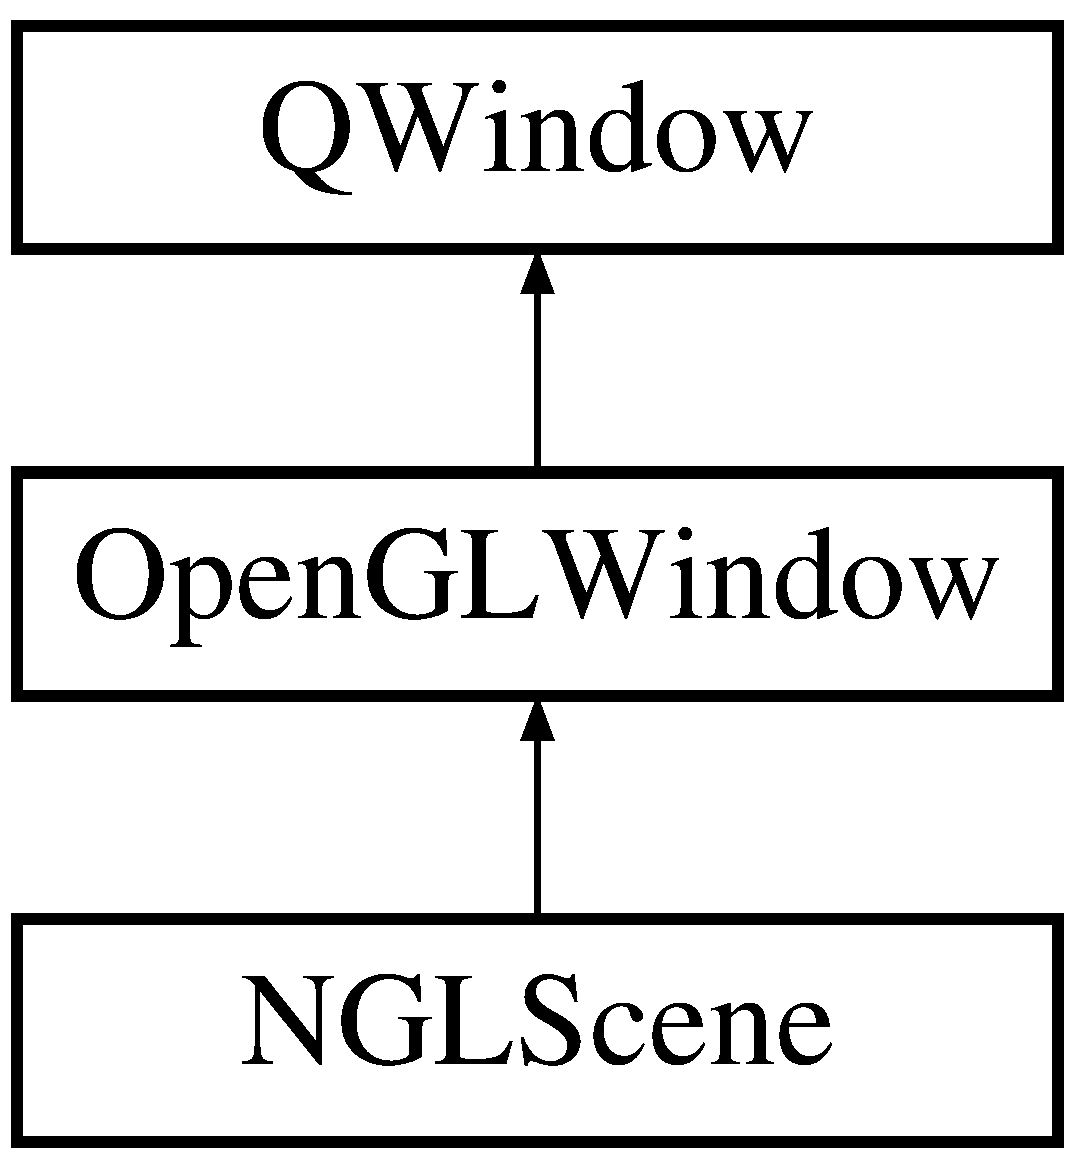
\includegraphics[height=3.000000cm]{classNGLScene}
\end{center}
\end{figure}
\subsection*{Public Member Functions}
\begin{DoxyCompactItemize}
\item 
\hyperlink{classNGLScene_adbde5986bed766df177e33baa7fbb222}{N\-G\-L\-Scene} (Q\-Window $\ast$\-\_\-parent=0)
\begin{DoxyCompactList}\small\item\em ctor for our N\-G\-L drawing class \end{DoxyCompactList}\item 
\hypertarget{classNGLScene_abda05d130945833bfbb6bad8d619f7f5}{\hyperlink{classNGLScene_abda05d130945833bfbb6bad8d619f7f5}{$\sim$\-N\-G\-L\-Scene} ()}\label{classNGLScene_abda05d130945833bfbb6bad8d619f7f5}

\begin{DoxyCompactList}\small\item\em dtor must close down ngl and release Open\-G\-L resources \end{DoxyCompactList}\item 
\hypertarget{classNGLScene_a63e57fc201b639e51c6eed6ec3b6b992}{void \hyperlink{classNGLScene_a63e57fc201b639e51c6eed6ec3b6b992}{initialize} ()}\label{classNGLScene_a63e57fc201b639e51c6eed6ec3b6b992}

\begin{DoxyCompactList}\small\item\em the initialize class is called once when the window is created and we have a valid G\-L context use this to setup any default G\-L stuff \end{DoxyCompactList}\item 
\hypertarget{classNGLScene_a63905ed5bab957d8e2d5528f942feb42}{void \hyperlink{classNGLScene_a63905ed5bab957d8e2d5528f942feb42}{render} ()}\label{classNGLScene_a63905ed5bab957d8e2d5528f942feb42}

\begin{DoxyCompactList}\small\item\em this is called everytime we want to draw the scene \end{DoxyCompactList}\end{DoxyCompactItemize}
\subsection*{Additional Inherited Members}


\subsection{Detailed Description}
our main glwindow widget for N\-G\-L applications all drawing elements are put in this file 

\subsection{Constructor \& Destructor Documentation}
\hypertarget{classNGLScene_adbde5986bed766df177e33baa7fbb222}{\index{N\-G\-L\-Scene@{N\-G\-L\-Scene}!N\-G\-L\-Scene@{N\-G\-L\-Scene}}
\index{N\-G\-L\-Scene@{N\-G\-L\-Scene}!NGLScene@{N\-G\-L\-Scene}}
\subsubsection[{N\-G\-L\-Scene}]{\setlength{\rightskip}{0pt plus 5cm}N\-G\-L\-Scene\-::\-N\-G\-L\-Scene (
\begin{DoxyParamCaption}
\item[{Q\-Window $\ast$}]{\-\_\-parent = {\ttfamily 0}}
\end{DoxyParamCaption}
)}}\label{classNGLScene_adbde5986bed766df177e33baa7fbb222}


ctor for our N\-G\-L drawing class 


\begin{DoxyParams}[1]{Parameters}
\mbox{\tt in}  & {\em parent} & the parent window to the class \\
\hline
\end{DoxyParams}


The documentation for this class was generated from the following files\-:\begin{DoxyCompactItemize}
\item 
include/\hyperlink{NGLScene_8h}{N\-G\-L\-Scene.\-h}\item 
src/N\-G\-L\-Scene.\-cpp\end{DoxyCompactItemize}

\hypertarget{classOpenGLWindow}{\section{Open\-G\-L\-Window Class Reference}
\label{classOpenGLWindow}\index{Open\-G\-L\-Window@{Open\-G\-L\-Window}}
}
Inheritance diagram for Open\-G\-L\-Window\-:\begin{figure}[H]
\begin{center}
\leavevmode
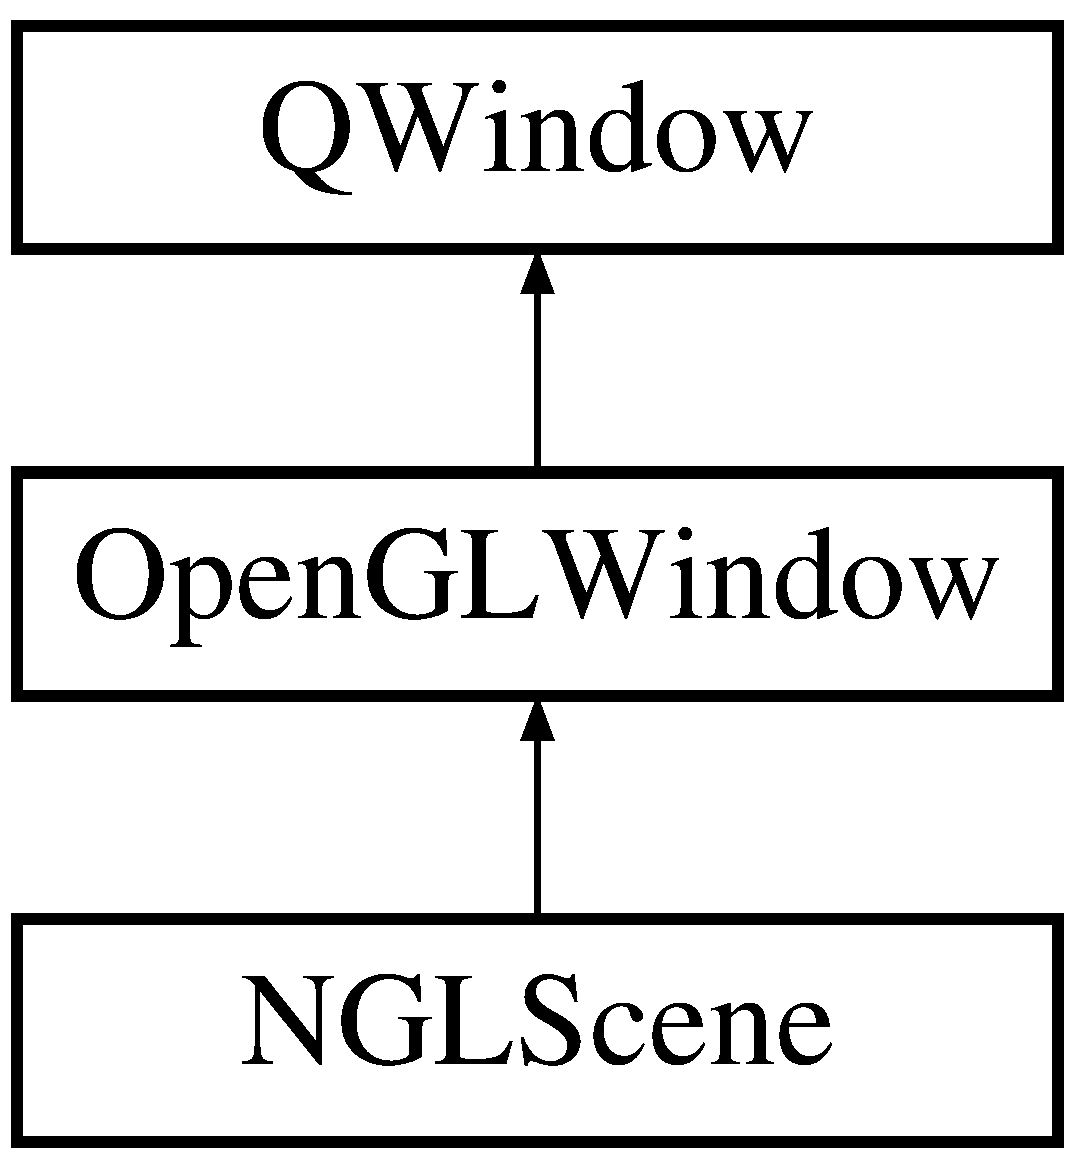
\includegraphics[height=3.000000cm]{classOpenGLWindow}
\end{center}
\end{figure}
\subsection*{Public Slots}
\begin{DoxyCompactItemize}
\item 
\hypertarget{classOpenGLWindow_abea9e50147496e5110b86f03122fbece}{void \hyperlink{classOpenGLWindow_abea9e50147496e5110b86f03122fbece}{render\-Later} ()}\label{classOpenGLWindow_abea9e50147496e5110b86f03122fbece}

\begin{DoxyCompactList}\small\item\em Qt slot to allow use to queue up a render for the next avaliable event process. \end{DoxyCompactList}\item 
\hypertarget{classOpenGLWindow_a8398ed62d646739fe54fae94c477ad1d}{void \hyperlink{classOpenGLWindow_a8398ed62d646739fe54fae94c477ad1d}{render\-Now} ()}\label{classOpenGLWindow_a8398ed62d646739fe54fae94c477ad1d}

\begin{DoxyCompactList}\small\item\em slot to tell us to render immediatly \end{DoxyCompactList}\end{DoxyCompactItemize}
\subsection*{Public Member Functions}
\begin{DoxyCompactItemize}
\item 
\hyperlink{classOpenGLWindow_a2fd92afd17361a60e058dc5433c316af}{Open\-G\-L\-Window} (Q\-Window $\ast$\-\_\-parent=0)
\begin{DoxyCompactList}\small\item\em ctor for Open\-G\-L window must set the surface type to Open\-G\-L \end{DoxyCompactList}\item 
\hypertarget{classOpenGLWindow_aa220b192c71871aab9100f4058a8d62d}{\hyperlink{classOpenGLWindow_aa220b192c71871aab9100f4058a8d62d}{$\sim$\-Open\-G\-L\-Window} ()}\label{classOpenGLWindow_aa220b192c71871aab9100f4058a8d62d}

\begin{DoxyCompactList}\small\item\em dtor, remember to remove the device once finished \end{DoxyCompactList}\item 
\hypertarget{classOpenGLWindow_a0e0194a4f0a30af7249819094c7d1d35}{virtual void \hyperlink{classOpenGLWindow_a0e0194a4f0a30af7249819094c7d1d35}{render} ()=0}\label{classOpenGLWindow_a0e0194a4f0a30af7249819094c7d1d35}

\begin{DoxyCompactList}\small\item\em pure virtual render method we override in our base class to do our drawing, called every update \end{DoxyCompactList}\item 
\hypertarget{classOpenGLWindow_a00b6a24198503b88aea4c5a995723db2}{virtual void \hyperlink{classOpenGLWindow_a00b6a24198503b88aea4c5a995723db2}{initialize} ()=0}\label{classOpenGLWindow_a00b6a24198503b88aea4c5a995723db2}

\begin{DoxyCompactList}\small\item\em pure virtual initialize method we override in our base class to do our drawing this is only called one time, just after we have a valid G\-L context use this to init any global G\-L elements \end{DoxyCompactList}\end{DoxyCompactItemize}
\subsection*{Protected Member Functions}
\begin{DoxyCompactItemize}
\item 
\hypertarget{classOpenGLWindow_a1e3045cffb900de55b7384f5091c9d94}{bool \hyperlink{classOpenGLWindow_a1e3045cffb900de55b7384f5091c9d94}{event} (Q\-Event $\ast$event)}\label{classOpenGLWindow_a1e3045cffb900de55b7384f5091c9d94}

\begin{DoxyCompactList}\small\item\em qt event processing if we post render\-Later event this will be called and execute a render \end{DoxyCompactList}\item 
\hypertarget{classOpenGLWindow_a991121ba7a4bbfa208fa74e5c86004c3}{void \hyperlink{classOpenGLWindow_a991121ba7a4bbfa208fa74e5c86004c3}{expose\-Event} (Q\-Expose\-Event $\ast$\hyperlink{classOpenGLWindow_a1e3045cffb900de55b7384f5091c9d94}{event})}\label{classOpenGLWindow_a991121ba7a4bbfa208fa74e5c86004c3}

\begin{DoxyCompactList}\small\item\em this even is called when the window is made visible and will trigger a render \end{DoxyCompactList}\end{DoxyCompactItemize}


\subsection{Constructor \& Destructor Documentation}
\hypertarget{classOpenGLWindow_a2fd92afd17361a60e058dc5433c316af}{\index{Open\-G\-L\-Window@{Open\-G\-L\-Window}!Open\-G\-L\-Window@{Open\-G\-L\-Window}}
\index{Open\-G\-L\-Window@{Open\-G\-L\-Window}!OpenGLWindow@{Open\-G\-L\-Window}}
\subsubsection[{Open\-G\-L\-Window}]{\setlength{\rightskip}{0pt plus 5cm}Open\-G\-L\-Window\-::\-Open\-G\-L\-Window (
\begin{DoxyParamCaption}
\item[{Q\-Window $\ast$}]{\-\_\-parent = {\ttfamily 0}}
\end{DoxyParamCaption}
)\hspace{0.3cm}{\ttfamily [explicit]}}}\label{classOpenGLWindow_a2fd92afd17361a60e058dc5433c316af}


ctor for Open\-G\-L window must set the surface type to Open\-G\-L 


\begin{DoxyParams}[1]{Parameters}
\mbox{\tt in}  & {\em parent} & the parent window to the class \\
\hline
\end{DoxyParams}


The documentation for this class was generated from the following files\-:\begin{DoxyCompactItemize}
\item 
include/\hyperlink{OpenGLWindow_8h}{Open\-G\-L\-Window.\-h}\item 
src/Open\-G\-L\-Window.\-cpp\end{DoxyCompactItemize}

\hypertarget{classparticle}{\section{particle Class Reference}
\label{classparticle}\index{particle@{particle}}
}


Our particle class.  




{\ttfamily \#include $<$particle.\-h$>$}

\subsection*{Public Member Functions}
\begin{DoxyCompactItemize}
\item 
\hyperlink{classparticle_a2849319f713e734cf009587505ba1075}{particle} (ngl\-::\-Vec3 $\ast$\-\_\-pos, float \-\_\-mass, bool \-\_\-part\-Of\-Mesh=false)
\begin{DoxyCompactList}\small\item\em our constructor to create our particle \end{DoxyCompactList}\item 
\hypertarget{classparticle_a6527e937e7db59e6edb6ae051c51866e}{\hyperlink{classparticle_a6527e937e7db59e6edb6ae051c51866e}{$\sim$particle} ()}\label{classparticle_a6527e937e7db59e6edb6ae051c51866e}

\begin{DoxyCompactList}\small\item\em default dtor \end{DoxyCompactList}\item 
\hypertarget{classparticle_ae6ee47584e0d79b3497ad2b906d764d5}{ngl\-::\-Vec3 \hyperlink{classparticle_ae6ee47584e0d79b3497ad2b906d764d5}{get\-Pos} () const }\label{classparticle_ae6ee47584e0d79b3497ad2b906d764d5}

\begin{DoxyCompactList}\small\item\em A function to return our particles position. \end{DoxyCompactList}\item 
\hypertarget{classparticle_abdcf2fa79e90f4b82c1d2eb5135e1322}{ngl\-::\-Vec3 \hyperlink{classparticle_abdcf2fa79e90f4b82c1d2eb5135e1322}{get\-Acc} () const }\label{classparticle_abdcf2fa79e90f4b82c1d2eb5135e1322}

\begin{DoxyCompactList}\small\item\em A function to return our particles Acceleration. \end{DoxyCompactList}\item 
\hypertarget{classparticle_a724a0799183e2a8f3665625187aaff30}{ngl\-::\-Vec3 \hyperlink{classparticle_a724a0799183e2a8f3665625187aaff30}{get\-Vel} () const }\label{classparticle_a724a0799183e2a8f3665625187aaff30}

\begin{DoxyCompactList}\small\item\em A function to return our particles velocity. \end{DoxyCompactList}\item 
\hypertarget{classparticle_ae5bff0edd62b18cabdd334b6d70d37a7}{float \hyperlink{classparticle_ae5bff0edd62b18cabdd334b6d70d37a7}{get\-Radius} () const }\label{classparticle_ae5bff0edd62b18cabdd334b6d70d37a7}

\begin{DoxyCompactList}\small\item\em A function to return the radius of our particle. \end{DoxyCompactList}\item 
void \hyperlink{classparticle_ab5e66d4d32f574767b9fd930224ae5ca}{set\-Pos} (ngl\-::\-Vec3 \-\_\-pos)
\begin{DoxyCompactList}\small\item\em A function to update our Postion once calculated. \end{DoxyCompactList}\item 
void \hyperlink{classparticle_a7802fa188578565fe14ae6701366e99e}{set\-Acc} (ngl\-::\-Vec3 \-\_\-acc)
\begin{DoxyCompactList}\small\item\em A function to update our Acceleration once calculated. \end{DoxyCompactList}\item 
void \hyperlink{classparticle_a63a467234510f284bb9a6ce9f3948be2}{set\-Vel} (ngl\-::\-Vec3 \-\_\-vel)
\begin{DoxyCompactList}\small\item\em A function to update our Velocity once calculated. \end{DoxyCompactList}\item 
void \hyperlink{classparticle_a2d12e2ddf643d3c3c9d76fbc37be76af}{set\-Mass} (float \-\_\-mass)
\begin{DoxyCompactList}\small\item\em sets the mass of our particle \end{DoxyCompactList}\item 
\hypertarget{classparticle_a9580ed056e4454fb9af79f98f2283497}{float \hyperlink{classparticle_a9580ed056e4454fb9af79f98f2283497}{get\-Mass} ()}\label{classparticle_a9580ed056e4454fb9af79f98f2283497}

\begin{DoxyCompactList}\small\item\em returns the mass of our particle \end{DoxyCompactList}\item 
void \hyperlink{classparticle_ab31fe756e1178e92cd4ee758635195ce}{set\-Density} (float \-\_\-density)
\begin{DoxyCompactList}\small\item\em sets the dynamic density of our particle \end{DoxyCompactList}\item 
\hypertarget{classparticle_a2cf7e7f0fbc93851a8c73cf824528968}{float \hyperlink{classparticle_a2cf7e7f0fbc93851a8c73cf824528968}{get\-Rest\-Density} ()}\label{classparticle_a2cf7e7f0fbc93851a8c73cf824528968}

\begin{DoxyCompactList}\small\item\em returns the rest density of our particle \end{DoxyCompactList}\item 
void \hyperlink{classparticle_a87171c315e8fe569d833a5bf26e22213}{set\-Rest\-Density} (float \-\_\-density)
\begin{DoxyCompactList}\small\item\em sets the rest density of our particle \end{DoxyCompactList}\item 
\hypertarget{classparticle_a48283e5e0e3fa83e19f7cfd286a863b1}{float \hyperlink{classparticle_a48283e5e0e3fa83e19f7cfd286a863b1}{get\-Density} ()}\label{classparticle_a48283e5e0e3fa83e19f7cfd286a863b1}

\begin{DoxyCompactList}\small\item\em returns the density of our particle \end{DoxyCompactList}\item 
void \hyperlink{classparticle_a6193659820dd29890c3319da28346658}{draw} (ngl\-::\-Transform\-Stack trans)
\begin{DoxyCompactList}\small\item\em draws our particles \end{DoxyCompactList}\item 
void \hyperlink{classparticle_a795f103cded87c05bf417f0b96adbbfd}{set\-Camera} (ngl\-::\-Camera $\ast$\-\_\-c)
\begin{DoxyCompactList}\small\item\em set our scenes camera so we know our V\-P matrices for drawing \end{DoxyCompactList}\end{DoxyCompactItemize}


\subsection{Detailed Description}
Our particle class. 

\subsection{Constructor \& Destructor Documentation}
\hypertarget{classparticle_a2849319f713e734cf009587505ba1075}{\index{particle@{particle}!particle@{particle}}
\index{particle@{particle}!particle@{particle}}
\subsubsection[{particle}]{\setlength{\rightskip}{0pt plus 5cm}particle\-::particle (
\begin{DoxyParamCaption}
\item[{ngl\-::\-Vec3 $\ast$}]{\-\_\-pos, }
\item[{float}]{\-\_\-mass, }
\item[{bool}]{\-\_\-part\-Of\-Mesh = {\ttfamily false}}
\end{DoxyParamCaption}
)}}\label{classparticle_a2849319f713e734cf009587505ba1075}


our constructor to create our particle 


\begin{DoxyParams}{Parameters}
{\em \-\_\-pos} & -\/ a ngl\-::vec3$\ast$ of the position of our particle \\
\hline
{\em \-\_\-mass} & -\/ the mass of our particle used for later calculations \\
\hline
{\em \-\_\-part\-Of\-Mesh} & -\/ if part of mesh will store a pointer to the vector location else will create a local one \\
\hline
\end{DoxyParams}


\subsection{Member Function Documentation}
\hypertarget{classparticle_a6193659820dd29890c3319da28346658}{\index{particle@{particle}!draw@{draw}}
\index{draw@{draw}!particle@{particle}}
\subsubsection[{draw}]{\setlength{\rightskip}{0pt plus 5cm}void particle\-::draw (
\begin{DoxyParamCaption}
\item[{ngl\-::\-Transform\-Stack}]{trans}
\end{DoxyParamCaption}
)}}\label{classparticle_a6193659820dd29890c3319da28346658}


draws our particles 


\begin{DoxyParams}{Parameters}
{\em trans} & -\/ our scenes transform stack to get our M matrix \\
\hline
\end{DoxyParams}
\hypertarget{classparticle_a7802fa188578565fe14ae6701366e99e}{\index{particle@{particle}!set\-Acc@{set\-Acc}}
\index{set\-Acc@{set\-Acc}!particle@{particle}}
\subsubsection[{set\-Acc}]{\setlength{\rightskip}{0pt plus 5cm}void particle\-::set\-Acc (
\begin{DoxyParamCaption}
\item[{ngl\-::\-Vec3}]{\-\_\-acc}
\end{DoxyParamCaption}
)\hspace{0.3cm}{\ttfamily [inline]}}}\label{classparticle_a7802fa188578565fe14ae6701366e99e}


A function to update our Acceleration once calculated. 


\begin{DoxyParams}{Parameters}
{\em \-\_\-acc} & the acceleration Vertext \\
\hline
\end{DoxyParams}
\hypertarget{classparticle_a795f103cded87c05bf417f0b96adbbfd}{\index{particle@{particle}!set\-Camera@{set\-Camera}}
\index{set\-Camera@{set\-Camera}!particle@{particle}}
\subsubsection[{set\-Camera}]{\setlength{\rightskip}{0pt plus 5cm}void particle\-::set\-Camera (
\begin{DoxyParamCaption}
\item[{ngl\-::\-Camera $\ast$}]{\-\_\-c}
\end{DoxyParamCaption}
)\hspace{0.3cm}{\ttfamily [inline]}}}\label{classparticle_a795f103cded87c05bf417f0b96adbbfd}


set our scenes camera so we know our V\-P matrices for drawing 


\begin{DoxyParams}{Parameters}
{\em our} & scenes camera \\
\hline
\end{DoxyParams}
\hypertarget{classparticle_ab31fe756e1178e92cd4ee758635195ce}{\index{particle@{particle}!set\-Density@{set\-Density}}
\index{set\-Density@{set\-Density}!particle@{particle}}
\subsubsection[{set\-Density}]{\setlength{\rightskip}{0pt plus 5cm}void particle\-::set\-Density (
\begin{DoxyParamCaption}
\item[{float}]{\-\_\-density}
\end{DoxyParamCaption}
)\hspace{0.3cm}{\ttfamily [inline]}}}\label{classparticle_ab31fe756e1178e92cd4ee758635195ce}


sets the dynamic density of our particle 


\begin{DoxyParams}{Parameters}
{\em \-\_\-density} & -\/ the density \\
\hline
\end{DoxyParams}
\hypertarget{classparticle_a2d12e2ddf643d3c3c9d76fbc37be76af}{\index{particle@{particle}!set\-Mass@{set\-Mass}}
\index{set\-Mass@{set\-Mass}!particle@{particle}}
\subsubsection[{set\-Mass}]{\setlength{\rightskip}{0pt plus 5cm}void particle\-::set\-Mass (
\begin{DoxyParamCaption}
\item[{float}]{\-\_\-mass}
\end{DoxyParamCaption}
)\hspace{0.3cm}{\ttfamily [inline]}}}\label{classparticle_a2d12e2ddf643d3c3c9d76fbc37be76af}


sets the mass of our particle 


\begin{DoxyParams}{Parameters}
{\em \-\_\-mass} & -\/ the mass \\
\hline
\end{DoxyParams}
\hypertarget{classparticle_ab5e66d4d32f574767b9fd930224ae5ca}{\index{particle@{particle}!set\-Pos@{set\-Pos}}
\index{set\-Pos@{set\-Pos}!particle@{particle}}
\subsubsection[{set\-Pos}]{\setlength{\rightskip}{0pt plus 5cm}void particle\-::set\-Pos (
\begin{DoxyParamCaption}
\item[{ngl\-::\-Vec3}]{\-\_\-pos}
\end{DoxyParamCaption}
)\hspace{0.3cm}{\ttfamily [inline]}}}\label{classparticle_ab5e66d4d32f574767b9fd930224ae5ca}


A function to update our Postion once calculated. 


\begin{DoxyParams}{Parameters}
{\em \-\_\-pos} & Vertex position \\
\hline
\end{DoxyParams}
\hypertarget{classparticle_a87171c315e8fe569d833a5bf26e22213}{\index{particle@{particle}!set\-Rest\-Density@{set\-Rest\-Density}}
\index{set\-Rest\-Density@{set\-Rest\-Density}!particle@{particle}}
\subsubsection[{set\-Rest\-Density}]{\setlength{\rightskip}{0pt plus 5cm}void particle\-::set\-Rest\-Density (
\begin{DoxyParamCaption}
\item[{float}]{\-\_\-density}
\end{DoxyParamCaption}
)\hspace{0.3cm}{\ttfamily [inline]}}}\label{classparticle_a87171c315e8fe569d833a5bf26e22213}


sets the rest density of our particle 


\begin{DoxyParams}{Parameters}
{\em \-\_\-density} & -\/ the rest density \\
\hline
\end{DoxyParams}
\hypertarget{classparticle_a63a467234510f284bb9a6ce9f3948be2}{\index{particle@{particle}!set\-Vel@{set\-Vel}}
\index{set\-Vel@{set\-Vel}!particle@{particle}}
\subsubsection[{set\-Vel}]{\setlength{\rightskip}{0pt plus 5cm}void particle\-::set\-Vel (
\begin{DoxyParamCaption}
\item[{ngl\-::\-Vec3}]{\-\_\-vel}
\end{DoxyParamCaption}
)\hspace{0.3cm}{\ttfamily [inline]}}}\label{classparticle_a63a467234510f284bb9a6ce9f3948be2}


A function to update our Velocity once calculated. 


\begin{DoxyParams}{Parameters}
{\em \-\_\-vel} & the Velocity Vertex \\
\hline
\end{DoxyParams}


The documentation for this class was generated from the following files\-:\begin{DoxyCompactItemize}
\item 
include/\hyperlink{particle_8h}{particle.\-h}\item 
src/particle.\-cpp\end{DoxyCompactItemize}

\hypertarget{classSPHHash}{\section{S\-P\-H\-Hash Class Reference}
\label{classSPHHash}\index{S\-P\-H\-Hash@{S\-P\-H\-Hash}}
}


Our hash class. this class will hash particles based on their position and return neighbours of the same key.  




{\ttfamily \#include $<$S\-P\-H\-Hash.\-h$>$}

\subsection*{Public Member Functions}
\begin{DoxyCompactItemize}
\item 
\hypertarget{classSPHHash_a932bc74f4bcb35b889c26264a1b6611f}{\hyperlink{classSPHHash_a932bc74f4bcb35b889c26264a1b6611f}{S\-P\-H\-Hash} ()}\label{classSPHHash_a932bc74f4bcb35b889c26264a1b6611f}

\begin{DoxyCompactList}\small\item\em default constructor \end{DoxyCompactList}\item 
\hypertarget{classSPHHash_a36ee41bd38353aae787b3e21db483bf0}{\hyperlink{classSPHHash_a36ee41bd38353aae787b3e21db483bf0}{$\sim$\-S\-P\-H\-Hash} ()}\label{classSPHHash_a36ee41bd38353aae787b3e21db483bf0}

\begin{DoxyCompactList}\small\item\em default destructor \end{DoxyCompactList}\item 
void \hyperlink{classSPHHash_a7f2a79b0f805eaec59261bcb4c152fe3}{set\-Prime} (int \-\_\-array\-Pos, double \-\_\-prime)
\begin{DoxyCompactList}\small\item\em mutator for our prime numbers if we want to set them to somthing else \end{DoxyCompactList}\item 
int \hyperlink{classSPHHash_a4e9e9732324d78090691c16a826ce0b4}{get\-Prime} (int \-\_\-array\-Pos)
\begin{DoxyCompactList}\small\item\em accessor for our prime numbers if we want to query them \end{DoxyCompactList}\item 
void \hyperlink{classSPHHash_abb619376308257ed514a52af3615ac96}{set\-Smoothing\-Length} (float \-\_\-smoothing\-Length)
\begin{DoxyCompactList}\small\item\em A mutatator for our smoothing length, h variable in navier stokes eqations. \end{DoxyCompactList}\item 
\hypertarget{classSPHHash_ad0de738a768a20c73a532a32aa09b64e}{float \hyperlink{classSPHHash_ad0de738a768a20c73a532a32aa09b64e}{get\-Smoothing\-Length} ()}\label{classSPHHash_ad0de738a768a20c73a532a32aa09b64e}

\begin{DoxyCompactList}\small\item\em returns our Smoothing Length if we need to query it \end{DoxyCompactList}\item 
void \hyperlink{classSPHHash_a2a4792b43ef215f7e2732cb77ea6e788}{create\-Hash\-Table} (std\-::vector$<$ \hyperlink{classparticle}{particle} $\ast$ $>$ \-\_\-particles)
\begin{DoxyCompactList}\small\item\em a function to fill our initially fill our hash table wil our particles \end{DoxyCompactList}\item 
std\-::vector$<$ \hyperlink{classparticle}{particle} $\ast$ $>$ \hyperlink{classSPHHash_a6d83b8f854980ef78d6e7e65c713074d}{get\-Neighbours} (\hyperlink{classparticle}{particle} $\ast$\-\_\-current\-Particle)
\begin{DoxyCompactList}\small\item\em Returns a vector of a particles neighbours. \end{DoxyCompactList}\item 
std\-::vector$<$ \hyperlink{classparticle}{particle} $\ast$ $>$ \hyperlink{classSPHHash_ab82b9de0e52cf1bd70cd508bdfd4f1c9}{get\-Neighbours} (\hyperlink{classparticle}{particle} $\ast$\-\_\-current\-Particle, int num\-Particles)
\begin{DoxyCompactList}\small\item\em Returns a vector of a limited number of particles neighbours, used for optimization. \end{DoxyCompactList}\end{DoxyCompactItemize}
\subsection*{Protected Member Functions}
\begin{DoxyCompactItemize}
\item 
int \hyperlink{classSPHHash_a3c4deda30ec87a73d29f6c0b949dd61e}{hash\-Function} (\hyperlink{classparticle}{particle} $\ast$\-\_\-particle)
\begin{DoxyCompactList}\small\item\em Hash function that generates a key based on the particle position. \end{DoxyCompactList}\item 
int \hyperlink{classSPHHash_a3a8bfb900e3f8939134b68d992a4e44b}{next\-Prime\-Num} (int \-\_\-current\-Num)
\begin{DoxyCompactList}\small\item\em A simple function that returns the next prime number from an input number. This is used in calculating our hash. \end{DoxyCompactList}\end{DoxyCompactItemize}


\subsection{Detailed Description}
Our hash class. this class will hash particles based on their position and return neighbours of the same key. 

\subsection{Member Function Documentation}
\hypertarget{classSPHHash_a2a4792b43ef215f7e2732cb77ea6e788}{\index{S\-P\-H\-Hash@{S\-P\-H\-Hash}!create\-Hash\-Table@{create\-Hash\-Table}}
\index{create\-Hash\-Table@{create\-Hash\-Table}!SPHHash@{S\-P\-H\-Hash}}
\subsubsection[{create\-Hash\-Table}]{\setlength{\rightskip}{0pt plus 5cm}void S\-P\-H\-Hash\-::create\-Hash\-Table (
\begin{DoxyParamCaption}
\item[{std\-::vector$<$ {\bf particle} $\ast$ $>$}]{\-\_\-particles}
\end{DoxyParamCaption}
)}}\label{classSPHHash_a2a4792b43ef215f7e2732cb77ea6e788}


a function to fill our initially fill our hash table wil our particles 


\begin{DoxyParams}{Parameters}
{\em \-\_\-particles} & -\/ the vector of our particles \\
\hline
\end{DoxyParams}
\hypertarget{classSPHHash_a6d83b8f854980ef78d6e7e65c713074d}{\index{S\-P\-H\-Hash@{S\-P\-H\-Hash}!get\-Neighbours@{get\-Neighbours}}
\index{get\-Neighbours@{get\-Neighbours}!SPHHash@{S\-P\-H\-Hash}}
\subsubsection[{get\-Neighbours}]{\setlength{\rightskip}{0pt plus 5cm}std\-::vector$<$ {\bf particle} $\ast$ $>$ S\-P\-H\-Hash\-::get\-Neighbours (
\begin{DoxyParamCaption}
\item[{{\bf particle} $\ast$}]{\-\_\-current\-Particle}
\end{DoxyParamCaption}
)}}\label{classSPHHash_a6d83b8f854980ef78d6e7e65c713074d}


Returns a vector of a particles neighbours. 


\begin{DoxyParams}{Parameters}
{\em \-\_\-current\-Particle} & -\/ the particle we want to ind the neighbours of \\
\hline
\end{DoxyParams}
\begin{DoxyReturn}{Returns}
vector of particle neighbours to our current particles 
\end{DoxyReturn}
\hypertarget{classSPHHash_ab82b9de0e52cf1bd70cd508bdfd4f1c9}{\index{S\-P\-H\-Hash@{S\-P\-H\-Hash}!get\-Neighbours@{get\-Neighbours}}
\index{get\-Neighbours@{get\-Neighbours}!SPHHash@{S\-P\-H\-Hash}}
\subsubsection[{get\-Neighbours}]{\setlength{\rightskip}{0pt plus 5cm}std\-::vector$<$ {\bf particle} $\ast$ $>$ S\-P\-H\-Hash\-::get\-Neighbours (
\begin{DoxyParamCaption}
\item[{{\bf particle} $\ast$}]{\-\_\-current\-Particle, }
\item[{int}]{num\-Particles}
\end{DoxyParamCaption}
)}}\label{classSPHHash_ab82b9de0e52cf1bd70cd508bdfd4f1c9}


Returns a vector of a limited number of particles neighbours, used for optimization. 


\begin{DoxyParams}{Parameters}
{\em \-\_\-current\-Particle} & -\/ the particle we want to ind the neighbours of \\
\hline
{\em num\-Particles} & -\/ the max number of particles you want to sample \\
\hline
\end{DoxyParams}
\begin{DoxyReturn}{Returns}
num\-Particle amount or neighbours to our current particle 
\end{DoxyReturn}
\hypertarget{classSPHHash_a4e9e9732324d78090691c16a826ce0b4}{\index{S\-P\-H\-Hash@{S\-P\-H\-Hash}!get\-Prime@{get\-Prime}}
\index{get\-Prime@{get\-Prime}!SPHHash@{S\-P\-H\-Hash}}
\subsubsection[{get\-Prime}]{\setlength{\rightskip}{0pt plus 5cm}int S\-P\-H\-Hash\-::get\-Prime (
\begin{DoxyParamCaption}
\item[{int}]{\-\_\-array\-Pos}
\end{DoxyParamCaption}
)\hspace{0.3cm}{\ttfamily [inline]}}}\label{classSPHHash_a4e9e9732324d78090691c16a826ce0b4}


accessor for our prime numbers if we want to query them 


\begin{DoxyParams}{Parameters}
{\em \-\_\-array\-Pos} & -\/ the position of the array that holds the 3 prime numbers \\
\hline
\end{DoxyParams}
\hypertarget{classSPHHash_a3c4deda30ec87a73d29f6c0b949dd61e}{\index{S\-P\-H\-Hash@{S\-P\-H\-Hash}!hash\-Function@{hash\-Function}}
\index{hash\-Function@{hash\-Function}!SPHHash@{S\-P\-H\-Hash}}
\subsubsection[{hash\-Function}]{\setlength{\rightskip}{0pt plus 5cm}int S\-P\-H\-Hash\-::hash\-Function (
\begin{DoxyParamCaption}
\item[{{\bf particle} $\ast$}]{\-\_\-particle}
\end{DoxyParamCaption}
)\hspace{0.3cm}{\ttfamily [protected]}}}\label{classSPHHash_a3c4deda30ec87a73d29f6c0b949dd61e}


Hash function that generates a key based on the particle position. 


\begin{DoxyParams}{Parameters}
{\em \-\_\-particle} & -\/ the particle we want to create the key for \\
\hline
\end{DoxyParams}
\hypertarget{classSPHHash_a3a8bfb900e3f8939134b68d992a4e44b}{\index{S\-P\-H\-Hash@{S\-P\-H\-Hash}!next\-Prime\-Num@{next\-Prime\-Num}}
\index{next\-Prime\-Num@{next\-Prime\-Num}!SPHHash@{S\-P\-H\-Hash}}
\subsubsection[{next\-Prime\-Num}]{\setlength{\rightskip}{0pt plus 5cm}int S\-P\-H\-Hash\-::next\-Prime\-Num (
\begin{DoxyParamCaption}
\item[{int}]{\-\_\-current\-Num}
\end{DoxyParamCaption}
)\hspace{0.3cm}{\ttfamily [protected]}}}\label{classSPHHash_a3a8bfb900e3f8939134b68d992a4e44b}


A simple function that returns the next prime number from an input number. This is used in calculating our hash. 


\begin{DoxyParams}{Parameters}
{\em \-\_\-current\-Num} & -\/ the number you want to calclate for \\
\hline
\end{DoxyParams}
\hypertarget{classSPHHash_a7f2a79b0f805eaec59261bcb4c152fe3}{\index{S\-P\-H\-Hash@{S\-P\-H\-Hash}!set\-Prime@{set\-Prime}}
\index{set\-Prime@{set\-Prime}!SPHHash@{S\-P\-H\-Hash}}
\subsubsection[{set\-Prime}]{\setlength{\rightskip}{0pt plus 5cm}void S\-P\-H\-Hash\-::set\-Prime (
\begin{DoxyParamCaption}
\item[{int}]{\-\_\-array\-Pos, }
\item[{double}]{\-\_\-prime}
\end{DoxyParamCaption}
)\hspace{0.3cm}{\ttfamily [inline]}}}\label{classSPHHash_a7f2a79b0f805eaec59261bcb4c152fe3}


mutator for our prime numbers if we want to set them to somthing else 


\begin{DoxyParams}{Parameters}
{\em \-\_\-array\-Pos} & -\/ position of the array that holds the 3 prime numbers \\
\hline
{\em \-\_\-prime} & -\/ the number you want to set it to \\
\hline
\end{DoxyParams}
\hypertarget{classSPHHash_abb619376308257ed514a52af3615ac96}{\index{S\-P\-H\-Hash@{S\-P\-H\-Hash}!set\-Smoothing\-Length@{set\-Smoothing\-Length}}
\index{set\-Smoothing\-Length@{set\-Smoothing\-Length}!SPHHash@{S\-P\-H\-Hash}}
\subsubsection[{set\-Smoothing\-Length}]{\setlength{\rightskip}{0pt plus 5cm}void S\-P\-H\-Hash\-::set\-Smoothing\-Length (
\begin{DoxyParamCaption}
\item[{float}]{\-\_\-smoothing\-Length}
\end{DoxyParamCaption}
)\hspace{0.3cm}{\ttfamily [inline]}}}\label{classSPHHash_abb619376308257ed514a52af3615ac96}


A mutatator for our smoothing length, h variable in navier stokes eqations. 


\begin{DoxyParams}{Parameters}
{\em \-\_\-smoothing\-Length} & -\/ the smoothing length \\
\hline
\end{DoxyParams}


The documentation for this class was generated from the following files\-:\begin{DoxyCompactItemize}
\item 
include/\hyperlink{SPHHash_8h}{S\-P\-H\-Hash.\-h}\item 
src/S\-P\-H\-Hash.\-cpp\end{DoxyCompactItemize}

\hypertarget{classSPHMelt}{\section{S\-P\-H\-Melt Class Reference}
\label{classSPHMelt}\index{S\-P\-H\-Melt@{S\-P\-H\-Melt}}
}


Our main simulation class. Used to call all the other classes we have created.  




{\ttfamily \#include $<$S\-P\-H\-Melt.\-h$>$}

\subsection*{Classes}
\begin{DoxyCompactItemize}
\item 
struct \hyperlink{structSPHMelt_1_1externalForce}{external\-Force}
\item 
struct \hyperlink{structSPHMelt_1_1vertData}{vert\-Data}
\end{DoxyCompactItemize}
\subsection*{Public Member Functions}
\begin{DoxyCompactItemize}
\item 
\hypertarget{classSPHMelt_abf63f796e20c65ea0792f3b57e9853c5}{\hyperlink{classSPHMelt_abf63f796e20c65ea0792f3b57e9853c5}{S\-P\-H\-Melt} ()}\label{classSPHMelt_abf63f796e20c65ea0792f3b57e9853c5}

\begin{DoxyCompactList}\small\item\em just a plain constructor that does nothing \end{DoxyCompactList}\item 
\hypertarget{classSPHMelt_af6fd66dad40740d7bb0af19ecfb650ea}{\hyperlink{classSPHMelt_af6fd66dad40740d7bb0af19ecfb650ea}{S\-P\-H\-Melt} (std\-::string \-\_\-mesh\-Location)}\label{classSPHMelt_af6fd66dad40740d7bb0af19ecfb650ea}

\begin{DoxyCompactList}\small\item\em Our constructor, reads in the vetexes of our mesh and stores them in m\-\_\-mesh\-Verts. \end{DoxyCompactList}\item 
\hypertarget{classSPHMelt_ac09f46a167ba1ce51e639eca54c2bc2a}{void \hyperlink{classSPHMelt_ac09f46a167ba1ce51e639eca54c2bc2a}{update} ()}\label{classSPHMelt_ac09f46a167ba1ce51e639eca54c2bc2a}

\begin{DoxyCompactList}\small\item\em Our update function. Update particles with S\-P\-H, Collision and then rewrites to the V\-A\-O. \end{DoxyCompactList}\item 
\hypertarget{classSPHMelt_a85a717d732a3e4be89d36cedb483d2ac}{void \hyperlink{classSPHMelt_a85a717d732a3e4be89d36cedb483d2ac}{draw\-Mesh} ()}\label{classSPHMelt_a85a717d732a3e4be89d36cedb483d2ac}

\begin{DoxyCompactList}\small\item\em A functio to draw our mesh. \end{DoxyCompactList}\item 
void \hyperlink{classSPHMelt_a64183bc720941736a9e3705fb896c993}{gen\-Particles} (int \-\_\-num\-Particles, float \-\_\-mass)
\begin{DoxyCompactList}\small\item\em A function to create our particles from our mesh vertecies. \end{DoxyCompactList}\item 
\hypertarget{classSPHMelt_a3d9da7029661124e3aabd1e24befa29d}{int \hyperlink{classSPHMelt_a3d9da7029661124e3aabd1e24befa29d}{get\-Num\-Particles} ()}\label{classSPHMelt_a3d9da7029661124e3aabd1e24befa29d}

\begin{DoxyCompactList}\small\item\em Just a fucntion so the scene can queury how many particles so that we can write it to screen. \end{DoxyCompactList}\item 
\hypertarget{classSPHMelt_a85546245558ea9821928e9b22470db52}{void \hyperlink{classSPHMelt_a85546245558ea9821928e9b22470db52}{init} ()}\label{classSPHMelt_a85546245558ea9821928e9b22470db52}

\begin{DoxyCompactList}\small\item\em Initialize our simulation. Set up V\-A\-O, generate particles, add collision walls and start the clock. \end{DoxyCompactList}\item 
void \hyperlink{classSPHMelt_ae1a307a3d8c33ebe599b74ab5bc2687c}{set\-Mesh\-Verts} (std\-::vector$<$ ngl\-::\-Vec3 $>$ \-\_\-vertex)
\begin{DoxyCompactList}\small\item\em we need a special function to convert the mesh vec3's to our vec3$\ast$ \end{DoxyCompactList}\item 
void \hyperlink{classSPHMelt_a47fbcb7522dbd8e647f818d094002d91}{set\-Cam} (ngl\-::\-Camera $\ast$\-\_\-c)
\begin{DoxyCompactList}\small\item\em set the scenes camera for all our particles \end{DoxyCompactList}\item 
void \hyperlink{classSPHMelt_a3293b79bb29229004db2b12d24f50778}{draw\-Particles} (ngl\-::\-Transform\-Stack trans)
\begin{DoxyCompactList}\small\item\em calls draw function in all our particles \end{DoxyCompactList}\item 
\hypertarget{classSPHMelt_a13d4145dbc7f7de93fd806a8971fe935}{void \hyperlink{classSPHMelt_a13d4145dbc7f7de93fd806a8971fe935}{reset\-Clock} ()}\label{classSPHMelt_a13d4145dbc7f7de93fd806a8971fe935}

\begin{DoxyCompactList}\small\item\em reset our clock. used if we pause the simulation \end{DoxyCompactList}\item 
\hypertarget{classSPHMelt_a2b67bc2d7444505213431381a1d96f55}{void \hyperlink{classSPHMelt_a2b67bc2d7444505213431381a1d96f55}{set\-External\-Force} (ngl\-::\-Vec3 \-\_\-source\-Pos=ngl\-::\-Vec3(0), float \-\_\-radius=0, float \-\_\-force\-Strength=0, bool \-\_\-push=true)}\label{classSPHMelt_a2b67bc2d7444505213431381a1d96f55}

\begin{DoxyCompactList}\small\item\em a fucntion to set the parameters of our external force for our S\-P\-H solver; \end{DoxyCompactList}\item 
void \hyperlink{classSPHMelt_a9286b6a873a0103ef13b2bc163bd75d2}{draw\-External\-Force} (ngl\-::\-Transform\-Stack $\ast$\-\_\-transform\-Stack, ngl\-::\-Camera $\ast$\-\_\-cam)
\begin{DoxyCompactList}\small\item\em a function to draw the source of our external force. \end{DoxyCompactList}\item 
void \hyperlink{classSPHMelt_ad291297d1b9c634b82ae5d033d9eb919}{draw\-Collision} (ngl\-::\-Transform\-Stack $\ast$\-\_\-transform\-Stack, ngl\-::\-Camera $\ast$\-\_\-cam)
\begin{DoxyCompactList}\small\item\em a function to draw the walls of our collision. Just used to pass paramiters to our collision class \end{DoxyCompactList}\item 
\hypertarget{classSPHMelt_a7922b30c46531e98ea6bbfa6ac51aa2a}{void \hyperlink{classSPHMelt_a7922b30c46531e98ea6bbfa6ac51aa2a}{start\-Mesh\-Sim} ()}\label{classSPHMelt_a7922b30c46531e98ea6bbfa6ac51aa2a}

\begin{DoxyCompactList}\small\item\em restarts the mesh simulation. \end{DoxyCompactList}\item 
\hypertarget{classSPHMelt_ab4ea1cf0ac6cec3828b296229505d4a6}{void \hyperlink{classSPHMelt_ab4ea1cf0ac6cec3828b296229505d4a6}{toggle\-Sim} ()}\label{classSPHMelt_ab4ea1cf0ac6cec3828b296229505d4a6}

\begin{DoxyCompactList}\small\item\em A function to toggle between our mesh simulation and our 2d simulation;. \end{DoxyCompactList}\item 
\hypertarget{classSPHMelt_a7645dc2f671f164fc288b2e0a6c0be37}{void \hyperlink{classSPHMelt_a7645dc2f671f164fc288b2e0a6c0be37}{restart} ()}\label{classSPHMelt_a7645dc2f671f164fc288b2e0a6c0be37}

\begin{DoxyCompactList}\small\item\em restarts the simumaltion \end{DoxyCompactList}\item 
\hypertarget{classSPHMelt_a3765b15c184fc6bda80fecdb43cfb287}{void \hyperlink{classSPHMelt_a3765b15c184fc6bda80fecdb43cfb287}{two\-D\-Water\-Sim\-Start} ()}\label{classSPHMelt_a3765b15c184fc6bda80fecdb43cfb287}

\begin{DoxyCompactList}\small\item\em change the scene to a 2d water simulation so you can see the physics \end{DoxyCompactList}\end{DoxyCompactItemize}


\subsection{Detailed Description}
Our main simulation class. Used to call all the other classes we have created. 

\subsection{Member Function Documentation}
\hypertarget{classSPHMelt_ad291297d1b9c634b82ae5d033d9eb919}{\index{S\-P\-H\-Melt@{S\-P\-H\-Melt}!draw\-Collision@{draw\-Collision}}
\index{draw\-Collision@{draw\-Collision}!SPHMelt@{S\-P\-H\-Melt}}
\subsubsection[{draw\-Collision}]{\setlength{\rightskip}{0pt plus 5cm}void S\-P\-H\-Melt\-::draw\-Collision (
\begin{DoxyParamCaption}
\item[{ngl\-::\-Transform\-Stack $\ast$}]{\-\_\-transform\-Stack, }
\item[{ngl\-::\-Camera $\ast$}]{\-\_\-cam}
\end{DoxyParamCaption}
)\hspace{0.3cm}{\ttfamily [inline]}}}\label{classSPHMelt_ad291297d1b9c634b82ae5d033d9eb919}


a function to draw the walls of our collision. Just used to pass paramiters to our collision class 


\begin{DoxyParams}{Parameters}
{\em \-\_\-transform\-Stack} & -\/ Our global transform stack so that they can rotate with the scene \\
\hline
{\em \-\_\-cam} & -\/ our scene camera so we can rotate the walls with the scene \\
\hline
\end{DoxyParams}
\hypertarget{classSPHMelt_a9286b6a873a0103ef13b2bc163bd75d2}{\index{S\-P\-H\-Melt@{S\-P\-H\-Melt}!draw\-External\-Force@{draw\-External\-Force}}
\index{draw\-External\-Force@{draw\-External\-Force}!SPHMelt@{S\-P\-H\-Melt}}
\subsubsection[{draw\-External\-Force}]{\setlength{\rightskip}{0pt plus 5cm}void S\-P\-H\-Melt\-::draw\-External\-Force (
\begin{DoxyParamCaption}
\item[{ngl\-::\-Transform\-Stack $\ast$}]{\-\_\-transform\-Stack, }
\item[{ngl\-::\-Camera $\ast$}]{\-\_\-cam}
\end{DoxyParamCaption}
)}}\label{classSPHMelt_a9286b6a873a0103ef13b2bc163bd75d2}


a function to draw the source of our external force. 


\begin{DoxyParams}{Parameters}
{\em \-\_\-transform\-Stack} & -\/ Our global transform stack so that they can rotate with the scene \\
\hline
{\em \-\_\-cam} & -\/ our scene camera so we can rotate with the scene \\
\hline
\end{DoxyParams}
\hypertarget{classSPHMelt_a3293b79bb29229004db2b12d24f50778}{\index{S\-P\-H\-Melt@{S\-P\-H\-Melt}!draw\-Particles@{draw\-Particles}}
\index{draw\-Particles@{draw\-Particles}!SPHMelt@{S\-P\-H\-Melt}}
\subsubsection[{draw\-Particles}]{\setlength{\rightskip}{0pt plus 5cm}void S\-P\-H\-Melt\-::draw\-Particles (
\begin{DoxyParamCaption}
\item[{ngl\-::\-Transform\-Stack}]{trans}
\end{DoxyParamCaption}
)}}\label{classSPHMelt_a3293b79bb29229004db2b12d24f50778}


calls draw function in all our particles 


\begin{DoxyParams}{Parameters}
{\em trans} & -\/ the transformstack of our scene \\
\hline
\end{DoxyParams}
\hypertarget{classSPHMelt_a64183bc720941736a9e3705fb896c993}{\index{S\-P\-H\-Melt@{S\-P\-H\-Melt}!gen\-Particles@{gen\-Particles}}
\index{gen\-Particles@{gen\-Particles}!SPHMelt@{S\-P\-H\-Melt}}
\subsubsection[{gen\-Particles}]{\setlength{\rightskip}{0pt plus 5cm}void S\-P\-H\-Melt\-::gen\-Particles (
\begin{DoxyParamCaption}
\item[{int}]{\-\_\-num\-Particles, }
\item[{float}]{\-\_\-mass}
\end{DoxyParamCaption}
)}}\label{classSPHMelt_a64183bc720941736a9e3705fb896c993}


A function to create our particles from our mesh vertecies. 


\begin{DoxyParams}{Parameters}
{\em \-\_\-num\-Particles} & -\/ The number of particles we want to create. If more than mesh verticies it will generate particles inside the mesh \\
\hline
\end{DoxyParams}
\begin{DoxyWarning}{Warning}
You must initialise the mesh first 
\end{DoxyWarning}
\hypertarget{classSPHMelt_a47fbcb7522dbd8e647f818d094002d91}{\index{S\-P\-H\-Melt@{S\-P\-H\-Melt}!set\-Cam@{set\-Cam}}
\index{set\-Cam@{set\-Cam}!SPHMelt@{S\-P\-H\-Melt}}
\subsubsection[{set\-Cam}]{\setlength{\rightskip}{0pt plus 5cm}void S\-P\-H\-Melt\-::set\-Cam (
\begin{DoxyParamCaption}
\item[{ngl\-::\-Camera $\ast$}]{\-\_\-c}
\end{DoxyParamCaption}
)}}\label{classSPHMelt_a47fbcb7522dbd8e647f818d094002d91}


set the scenes camera for all our particles 


\begin{DoxyParams}{Parameters}
{\em Our} & scenes particles \\
\hline
\end{DoxyParams}
\hypertarget{classSPHMelt_ae1a307a3d8c33ebe599b74ab5bc2687c}{\index{S\-P\-H\-Melt@{S\-P\-H\-Melt}!set\-Mesh\-Verts@{set\-Mesh\-Verts}}
\index{set\-Mesh\-Verts@{set\-Mesh\-Verts}!SPHMelt@{S\-P\-H\-Melt}}
\subsubsection[{set\-Mesh\-Verts}]{\setlength{\rightskip}{0pt plus 5cm}void S\-P\-H\-Melt\-::set\-Mesh\-Verts (
\begin{DoxyParamCaption}
\item[{std\-::vector$<$ ngl\-::\-Vec3 $>$}]{\-\_\-vertex}
\end{DoxyParamCaption}
)}}\label{classSPHMelt_ae1a307a3d8c33ebe599b74ab5bc2687c}


we need a special function to convert the mesh vec3's to our vec3$\ast$ 


\begin{DoxyParams}{Parameters}
{\em \-\_\-vertex} & -\/ Takes in the obj verticies \\
\hline
\end{DoxyParams}


The documentation for this class was generated from the following files\-:\begin{DoxyCompactItemize}
\item 
include/\hyperlink{SPHMelt_8h}{S\-P\-H\-Melt.\-h}\item 
src/S\-P\-H\-Melt.\-cpp\end{DoxyCompactItemize}

\hypertarget{classSPHSolver}{\section{S\-P\-H\-Solver Class Reference}
\label{classSPHSolver}\index{S\-P\-H\-Solver@{S\-P\-H\-Solver}}
}


Our solver class used to calculate our new particle positions with S\-P\-H equations.  




{\ttfamily \#include $<$S\-P\-H\-Solver.\-h$>$}

\subsection*{Public Member Functions}
\begin{DoxyCompactItemize}
\item 
\hypertarget{classSPHSolver_abe3a0bdf9c42b4213944bc0332020e65}{\hyperlink{classSPHSolver_abe3a0bdf9c42b4213944bc0332020e65}{S\-P\-H\-Solver} ()}\label{classSPHSolver_abe3a0bdf9c42b4213944bc0332020e65}

\begin{DoxyCompactList}\small\item\em default ctor \end{DoxyCompactList}\item 
\hypertarget{classSPHSolver_a81a0ee1c05b649912faa1e9839f71883}{\hyperlink{classSPHSolver_a81a0ee1c05b649912faa1e9839f71883}{$\sim$\-S\-P\-H\-Solver} ()}\label{classSPHSolver_a81a0ee1c05b649912faa1e9839f71883}

\begin{DoxyCompactList}\small\item\em default dtor \end{DoxyCompactList}\item 
void \hyperlink{classSPHSolver_ab7408071375d37e5455d90b53a02f444}{calc\-Forces} (\hyperlink{classparticle}{particle} $\ast$\-\_\-current\-Particle, std\-::vector$<$ \hyperlink{classparticle}{particle} $\ast$ $>$ \-\_\-particle\-Index, float \-\_\-time\-Step)
\begin{DoxyCompactList}\small\item\em Calculates the forces for a particle using leap frog method of integration. \end{DoxyCompactList}\item 
void \hyperlink{classSPHSolver_a27b0bebb170b2613a5ff0e681b64abe8}{calc\-Forces\-Euler} (\hyperlink{classparticle}{particle} $\ast$\-\_\-current\-Particle, std\-::vector$<$ \hyperlink{classparticle}{particle} $\ast$ $>$ \-\_\-particle\-Index, float \-\_\-time\-Step)
\begin{DoxyCompactList}\small\item\em Calculates the forces for a particle using Euler integration. \end{DoxyCompactList}\item 
void \hyperlink{classSPHSolver_a443a24a01177a91acb7a5c3e19d7283a}{set\-Smoothing\-Length} (float \-\_\-smoothing\-Length)
\begin{DoxyCompactList}\small\item\em A mutatator for our smoothing length, h variable in navier stokes eqations. \end{DoxyCompactList}\item 
\hypertarget{classSPHSolver_ab6f67635e1a6013adc6fa7e94312062d}{float \hyperlink{classSPHSolver_ab6f67635e1a6013adc6fa7e94312062d}{get\-Smoothing\-Length} ()}\label{classSPHSolver_ab6f67635e1a6013adc6fa7e94312062d}

\begin{DoxyCompactList}\small\item\em returns our Smoothing Length if we need to query it \end{DoxyCompactList}\item 
\hypertarget{classSPHSolver_a01c0580448eee39044bd624985cef25e}{void \hyperlink{classSPHSolver_a01c0580448eee39044bd624985cef25e}{set\-Vis\-Coef} (float \-\_\-x)}\label{classSPHSolver_a01c0580448eee39044bd624985cef25e}

\begin{DoxyCompactList}\small\item\em Set our viscosity coefficient for our navier stokes equations. \end{DoxyCompactList}\item 
void \hyperlink{classSPHSolver_aded0232e354909dfdb19ddc41e20bc7b}{init\-Density} (std\-::vector$<$ \hyperlink{classparticle}{particle} $\ast$ $>$ \-\_\-particle\-Index)
\begin{DoxyCompactList}\small\item\em Initialises the density for our particles. \end{DoxyCompactList}\item 
void \hyperlink{classSPHSolver_a62978b765c699c7e50a637ac17b8b64d}{set\-Gas\-Constant} (float \-\_\-x)
\begin{DoxyCompactList}\small\item\em set the gas constant for our water simulation \end{DoxyCompactList}\item 
void \hyperlink{classSPHSolver_ac1de32892a477c7474e06fc5bddfe24a}{set\-External\-Force} (ngl\-::\-Vec3 \-\_\-pos, float \-\_\-force\-Radius, float \-\_\-force\-Strength, bool \-\_\-push=true)
\begin{DoxyCompactList}\small\item\em Add an external force to our S\-P\-H calculations. acts like wind. \end{DoxyCompactList}\end{DoxyCompactItemize}
\subsection*{Protected Member Functions}
\begin{DoxyCompactItemize}
\item 
float \hyperlink{classSPHSolver_a70dd03e826824255b9fc76c67da53e19}{calc\-Density\-Kern} (\hyperlink{classparticle}{particle} $\ast$\-\_\-current\-Particle, \hyperlink{classparticle}{particle} $\ast$\-\_\-neighbour)
\begin{DoxyCompactList}\small\item\em calculates the smoothing kernal for density, used in our S\-P\-H equations \end{DoxyCompactList}\item 
ngl\-::\-Vec3 \hyperlink{classSPHSolver_a89a6fc730abeab6ae96c015ae9682ac1}{calc\-Pressure\-Kern} (\hyperlink{classparticle}{particle} $\ast$\-\_\-current\-Particle, \hyperlink{classparticle}{particle} $\ast$\-\_\-neighbour)
\begin{DoxyCompactList}\small\item\em calculates the smoothing kernal for density, used in our S\-P\-H equations \end{DoxyCompactList}\item 
ngl\-::\-Vec3 \hyperlink{classSPHSolver_a42e9c556eb3bfec29ef90c08545dff30}{calc\-Viscosity\-Kern} (\hyperlink{classparticle}{particle} $\ast$\-\_\-current\-Particle, \hyperlink{classparticle}{particle} $\ast$\-\_\-neighbour)
\begin{DoxyCompactList}\small\item\em calculates the smoothing kernal for density, used in our S\-P\-H equations \end{DoxyCompactList}\end{DoxyCompactItemize}


\subsection{Detailed Description}
Our solver class used to calculate our new particle positions with S\-P\-H equations. 

\subsection{Member Function Documentation}
\hypertarget{classSPHSolver_a70dd03e826824255b9fc76c67da53e19}{\index{S\-P\-H\-Solver@{S\-P\-H\-Solver}!calc\-Density\-Kern@{calc\-Density\-Kern}}
\index{calc\-Density\-Kern@{calc\-Density\-Kern}!SPHSolver@{S\-P\-H\-Solver}}
\subsubsection[{calc\-Density\-Kern}]{\setlength{\rightskip}{0pt plus 5cm}float S\-P\-H\-Solver\-::calc\-Density\-Kern (
\begin{DoxyParamCaption}
\item[{{\bf particle} $\ast$}]{\-\_\-current\-Particle, }
\item[{{\bf particle} $\ast$}]{\-\_\-neighbour}
\end{DoxyParamCaption}
)\hspace{0.3cm}{\ttfamily [protected]}}}\label{classSPHSolver_a70dd03e826824255b9fc76c67da53e19}


calculates the smoothing kernal for density, used in our S\-P\-H equations 


\begin{DoxyParams}{Parameters}
{\em \-\_\-current\-Particle} & the particle we wish to test for \\
\hline
{\em \-\_\-neighbour} & the particle we wish to test our \-\_\-current particle against \\
\hline
\end{DoxyParams}
\begin{DoxyReturn}{Returns}
the weight of influence the particle has on our \-\_\-current\-Particle 
\end{DoxyReturn}
\hypertarget{classSPHSolver_ab7408071375d37e5455d90b53a02f444}{\index{S\-P\-H\-Solver@{S\-P\-H\-Solver}!calc\-Forces@{calc\-Forces}}
\index{calc\-Forces@{calc\-Forces}!SPHSolver@{S\-P\-H\-Solver}}
\subsubsection[{calc\-Forces}]{\setlength{\rightskip}{0pt plus 5cm}void S\-P\-H\-Solver\-::calc\-Forces (
\begin{DoxyParamCaption}
\item[{{\bf particle} $\ast$}]{\-\_\-current\-Particle, }
\item[{std\-::vector$<$ {\bf particle} $\ast$ $>$}]{\-\_\-particle\-Index, }
\item[{float}]{\-\_\-time\-Step}
\end{DoxyParamCaption}
)}}\label{classSPHSolver_ab7408071375d37e5455d90b53a02f444}


Calculates the forces for a particle using leap frog method of integration. 


\begin{DoxyParams}{Parameters}
{\em \-\_\-current\-Particle} & -\/ The particle we are going to calculate the forces for \\
\hline
{\em \-\_\-particle\-Index} & -\/ Vector of all our particles if we want to brut force or the neighbour particles for S\-P\-H \\
\hline
{\em \-\_\-time\-Step} & -\/ the time step between updates \\
\hline
\end{DoxyParams}
\hypertarget{classSPHSolver_a27b0bebb170b2613a5ff0e681b64abe8}{\index{S\-P\-H\-Solver@{S\-P\-H\-Solver}!calc\-Forces\-Euler@{calc\-Forces\-Euler}}
\index{calc\-Forces\-Euler@{calc\-Forces\-Euler}!SPHSolver@{S\-P\-H\-Solver}}
\subsubsection[{calc\-Forces\-Euler}]{\setlength{\rightskip}{0pt plus 5cm}void S\-P\-H\-Solver\-::calc\-Forces\-Euler (
\begin{DoxyParamCaption}
\item[{{\bf particle} $\ast$}]{\-\_\-current\-Particle, }
\item[{std\-::vector$<$ {\bf particle} $\ast$ $>$}]{\-\_\-particle\-Index, }
\item[{float}]{\-\_\-time\-Step}
\end{DoxyParamCaption}
)}}\label{classSPHSolver_a27b0bebb170b2613a5ff0e681b64abe8}


Calculates the forces for a particle using Euler integration. 


\begin{DoxyParams}{Parameters}
{\em \-\_\-current\-Particle} & -\/ The particle we are going to calculate the forces for \\
\hline
{\em \-\_\-particle\-Index} & -\/ Vector of all our particles if we want to brut force or the neighbour particles for S\-P\-H \\
\hline
{\em \-\_\-time\-Step} & -\/ the time step between updates \\
\hline
\end{DoxyParams}
\hypertarget{classSPHSolver_a89a6fc730abeab6ae96c015ae9682ac1}{\index{S\-P\-H\-Solver@{S\-P\-H\-Solver}!calc\-Pressure\-Kern@{calc\-Pressure\-Kern}}
\index{calc\-Pressure\-Kern@{calc\-Pressure\-Kern}!SPHSolver@{S\-P\-H\-Solver}}
\subsubsection[{calc\-Pressure\-Kern}]{\setlength{\rightskip}{0pt plus 5cm}ngl\-::\-Vec3 S\-P\-H\-Solver\-::calc\-Pressure\-Kern (
\begin{DoxyParamCaption}
\item[{{\bf particle} $\ast$}]{\-\_\-current\-Particle, }
\item[{{\bf particle} $\ast$}]{\-\_\-neighbour}
\end{DoxyParamCaption}
)\hspace{0.3cm}{\ttfamily [protected]}}}\label{classSPHSolver_a89a6fc730abeab6ae96c015ae9682ac1}


calculates the smoothing kernal for density, used in our S\-P\-H equations 


\begin{DoxyParams}{Parameters}
{\em \-\_\-current\-Particle} & the particle we wish to test for \\
\hline
{\em \-\_\-neighbour} & the particle we wish to test our \-\_\-current particle against \\
\hline
\end{DoxyParams}
\begin{DoxyReturn}{Returns}
the weighted pressued gradient the particle has on our \-\_\-current\-Particle 
\end{DoxyReturn}
\hypertarget{classSPHSolver_a42e9c556eb3bfec29ef90c08545dff30}{\index{S\-P\-H\-Solver@{S\-P\-H\-Solver}!calc\-Viscosity\-Kern@{calc\-Viscosity\-Kern}}
\index{calc\-Viscosity\-Kern@{calc\-Viscosity\-Kern}!SPHSolver@{S\-P\-H\-Solver}}
\subsubsection[{calc\-Viscosity\-Kern}]{\setlength{\rightskip}{0pt plus 5cm}ngl\-::\-Vec3 S\-P\-H\-Solver\-::calc\-Viscosity\-Kern (
\begin{DoxyParamCaption}
\item[{{\bf particle} $\ast$}]{\-\_\-current\-Particle, }
\item[{{\bf particle} $\ast$}]{\-\_\-neighbour}
\end{DoxyParamCaption}
)\hspace{0.3cm}{\ttfamily [protected]}}}\label{classSPHSolver_a42e9c556eb3bfec29ef90c08545dff30}


calculates the smoothing kernal for density, used in our S\-P\-H equations 


\begin{DoxyParams}{Parameters}
{\em \-\_\-current\-Particle} & the particle we wish to test for \\
\hline
{\em \-\_\-neighbour} & the particle we wish to test our \-\_\-current particle against \\
\hline
\end{DoxyParams}
\begin{DoxyReturn}{Returns}
the weighted viscosity vector the particle has on our \-\_\-current\-Particle 
\end{DoxyReturn}
\hypertarget{classSPHSolver_aded0232e354909dfdb19ddc41e20bc7b}{\index{S\-P\-H\-Solver@{S\-P\-H\-Solver}!init\-Density@{init\-Density}}
\index{init\-Density@{init\-Density}!SPHSolver@{S\-P\-H\-Solver}}
\subsubsection[{init\-Density}]{\setlength{\rightskip}{0pt plus 5cm}void S\-P\-H\-Solver\-::init\-Density (
\begin{DoxyParamCaption}
\item[{std\-::vector$<$ {\bf particle} $\ast$ $>$}]{\-\_\-particle\-Index}
\end{DoxyParamCaption}
)}}\label{classSPHSolver_aded0232e354909dfdb19ddc41e20bc7b}


Initialises the density for our particles. 


\begin{DoxyParams}{Parameters}
{\em \-\_\-particle\-Index} & -\/ The vector of all our particles we want to initialize the density for \\
\hline
\end{DoxyParams}
\hypertarget{classSPHSolver_ac1de32892a477c7474e06fc5bddfe24a}{\index{S\-P\-H\-Solver@{S\-P\-H\-Solver}!set\-External\-Force@{set\-External\-Force}}
\index{set\-External\-Force@{set\-External\-Force}!SPHSolver@{S\-P\-H\-Solver}}
\subsubsection[{set\-External\-Force}]{\setlength{\rightskip}{0pt plus 5cm}void S\-P\-H\-Solver\-::set\-External\-Force (
\begin{DoxyParamCaption}
\item[{ngl\-::\-Vec3}]{\-\_\-pos, }
\item[{float}]{\-\_\-force\-Radius, }
\item[{float}]{\-\_\-force\-Strength, }
\item[{bool}]{\-\_\-push = {\ttfamily true}}
\end{DoxyParamCaption}
)\hspace{0.3cm}{\ttfamily [inline]}}}\label{classSPHSolver_ac1de32892a477c7474e06fc5bddfe24a}


Add an external force to our S\-P\-H calculations. acts like wind. 


\begin{DoxyParams}{Parameters}
{\em \-\_\-pos} & -\/ The source position of the force \\
\hline
{\em \-\_\-force\-Radius} & -\/ the area that the force has influence over. This has a linear falloff \\
\hline
{\em \-\_\-force\-Strength} & -\/ How strong your want your force to be. This is just a scaler. \\
\hline
{\em \-\_\-push} & -\/ a bool so we know weather we are pushing the particles away or sucking them towards us \\
\hline
\end{DoxyParams}
\hypertarget{classSPHSolver_a62978b765c699c7e50a637ac17b8b64d}{\index{S\-P\-H\-Solver@{S\-P\-H\-Solver}!set\-Gas\-Constant@{set\-Gas\-Constant}}
\index{set\-Gas\-Constant@{set\-Gas\-Constant}!SPHSolver@{S\-P\-H\-Solver}}
\subsubsection[{set\-Gas\-Constant}]{\setlength{\rightskip}{0pt plus 5cm}void S\-P\-H\-Solver\-::set\-Gas\-Constant (
\begin{DoxyParamCaption}
\item[{float}]{\-\_\-x}
\end{DoxyParamCaption}
)\hspace{0.3cm}{\ttfamily [inline]}}}\label{classSPHSolver_a62978b765c699c7e50a637ac17b8b64d}


set the gas constant for our water simulation 


\begin{DoxyParams}{Parameters}
{\em \-\_\-x} & -\/ the value we wish to set our constant to \\
\hline
\end{DoxyParams}
\hypertarget{classSPHSolver_a443a24a01177a91acb7a5c3e19d7283a}{\index{S\-P\-H\-Solver@{S\-P\-H\-Solver}!set\-Smoothing\-Length@{set\-Smoothing\-Length}}
\index{set\-Smoothing\-Length@{set\-Smoothing\-Length}!SPHSolver@{S\-P\-H\-Solver}}
\subsubsection[{set\-Smoothing\-Length}]{\setlength{\rightskip}{0pt plus 5cm}void S\-P\-H\-Solver\-::set\-Smoothing\-Length (
\begin{DoxyParamCaption}
\item[{float}]{\-\_\-smoothing\-Length}
\end{DoxyParamCaption}
)\hspace{0.3cm}{\ttfamily [inline]}}}\label{classSPHSolver_a443a24a01177a91acb7a5c3e19d7283a}


A mutatator for our smoothing length, h variable in navier stokes eqations. 


\begin{DoxyParams}{Parameters}
{\em \-\_\-smoothing\-Length} & -\/ the smoothing length \\
\hline
\end{DoxyParams}


The documentation for this class was generated from the following files\-:\begin{DoxyCompactItemize}
\item 
include/S\-P\-H\-Solver.\-h\item 
src/S\-P\-H\-Solver.\-cpp\end{DoxyCompactItemize}

\hypertarget{structSPHMelt_1_1vertData}{\section{S\-P\-H\-Melt\-:\-:vert\-Data Struct Reference}
\label{structSPHMelt_1_1vertData}\index{S\-P\-H\-Melt\-::vert\-Data@{S\-P\-H\-Melt\-::vert\-Data}}
}
\subsection*{Public Attributes}
\begin{DoxyCompactItemize}
\item 
\hypertarget{structSPHMelt_1_1vertData_a894467b3cd0fa8acd65fe42f661af100}{ngl\-::\-Vec3 {\bfseries p1}}\label{structSPHMelt_1_1vertData_a894467b3cd0fa8acd65fe42f661af100}

\item 
\hypertarget{structSPHMelt_1_1vertData_a997efb17fe5ea13a89103af57bd6c5dc}{ngl\-::\-Vec3 {\bfseries n1}}\label{structSPHMelt_1_1vertData_a997efb17fe5ea13a89103af57bd6c5dc}

\end{DoxyCompactItemize}


The documentation for this struct was generated from the following file\-:\begin{DoxyCompactItemize}
\item 
include/\hyperlink{SPHMelt_8h}{S\-P\-H\-Melt.\-h}\end{DoxyCompactItemize}

\chapter{File Documentation}
\hypertarget{NGLScene_8h}{\section{include/\-N\-G\-L\-Scene.h File Reference}
\label{NGLScene_8h}\index{include/\-N\-G\-L\-Scene.\-h@{include/\-N\-G\-L\-Scene.\-h}}
}


this class inherits from the Qt \hyperlink{classOpenGLWindow}{Open\-G\-L\-Window} and allows us to use N\-G\-L to draw Open\-G\-L  


{\ttfamily \#include \char`\"{}Open\-G\-L\-Window.\-h\char`\"{}}\\*
{\ttfamily \#include $<$ngl/\-Camera.\-h$>$}\\*
{\ttfamily \#include $<$ngl/\-Colour.\-h$>$}\\*
{\ttfamily \#include $<$ngl/\-Light.\-h$>$}\\*
{\ttfamily \#include $<$ngl/\-Obj.\-h$>$}\\*
{\ttfamily \#include $<$ngl/\-Transform\-Stack.\-h$>$}\\*
{\ttfamily \#include $<$ngl/\-Text.\-h$>$}\\*
{\ttfamily \#include $<$Q\-Timer$>$}\\*
{\ttfamily \#include $<$Q\-Time$>$}\\*
{\ttfamily \#include \char`\"{}S\-P\-H\-Melt.\-h\char`\"{}}\\*
\subsection*{Classes}
\begin{DoxyCompactItemize}
\item 
class \hyperlink{classNGLScene}{N\-G\-L\-Scene}
\begin{DoxyCompactList}\small\item\em our main glwindow widget for N\-G\-L applications all drawing elements are put in this file \end{DoxyCompactList}\end{DoxyCompactItemize}


\subsection{Detailed Description}
this class inherits from the Qt \hyperlink{classOpenGLWindow}{Open\-G\-L\-Window} and allows us to use N\-G\-L to draw Open\-G\-L \begin{DoxyAuthor}{Author}
Jonathan Macey 
\end{DoxyAuthor}
\begin{DoxyVersion}{Version}
1.\-0 
\end{DoxyVersion}
\begin{DoxyDate}{Date}
10/9/13 Revision History \-: This is an initial version used for the new N\-G\-L6 / Qt 5 demos 
\end{DoxyDate}

\hypertarget{OpenGLWindow_8h}{\section{include/\-Open\-G\-L\-Window.h File Reference}
\label{OpenGLWindow_8h}\index{include/\-Open\-G\-L\-Window.\-h@{include/\-Open\-G\-L\-Window.\-h}}
}


this is the base class for all our Open\-G\-L widgets, inherit from this class and overide the methods for Open\-G\-L drawing modified from the Qt demo here \href{http://qt-project.org/doc/qt-5.0/qtgui/openglwindow.html}{\tt http\-://qt-\/project.\-org/doc/qt-\/5.\-0/qtgui/openglwindow.\-html}  


{\ttfamily \#include $<$Qt\-Gui/\-Q\-Window$>$}\\*
\subsection*{Classes}
\begin{DoxyCompactItemize}
\item 
class \hyperlink{classOpenGLWindow}{Open\-G\-L\-Window}
\end{DoxyCompactItemize}


\subsection{Detailed Description}
this is the base class for all our Open\-G\-L widgets, inherit from this class and overide the methods for Open\-G\-L drawing modified from the Qt demo here \href{http://qt-project.org/doc/qt-5.0/qtgui/openglwindow.html}{\tt http\-://qt-\/project.\-org/doc/qt-\/5.\-0/qtgui/openglwindow.\-html} \begin{DoxyAuthor}{Author}
Jonathan Macey 
\end{DoxyAuthor}
\begin{DoxyVersion}{Version}
1.\-0 
\end{DoxyVersion}
\begin{DoxyDate}{Date}
10/9/13 Revision History \-: This is an initial version used for the new N\-G\-L6 / Qt 5 demos 
\end{DoxyDate}

\hypertarget{particle_8h}{\section{include/particle.h File Reference}
\label{particle_8h}\index{include/particle.\-h@{include/particle.\-h}}
}


Ths is my particle class, it will store all the data for my particles for my simulation.  


{\ttfamily \#include $<$ngl/\-Vec4.\-h$>$}\\*
{\ttfamily \#include $<$ngl/\-Camera.\-h$>$}\\*
{\ttfamily \#include $<$ngl/\-Transform\-Stack.\-h$>$}\\*
{\ttfamily \#include $<$ngl/\-V\-A\-O\-Primitives.\-h$>$}\\*
{\ttfamily \#include $<$ngl/\-Shader\-Lib.\-h$>$}\\*
\subsection*{Classes}
\begin{DoxyCompactItemize}
\item 
class \hyperlink{classparticle}{particle}
\begin{DoxyCompactList}\small\item\em Our particle class. \end{DoxyCompactList}\end{DoxyCompactItemize}


\subsection{Detailed Description}
Ths is my particle class, it will store all the data for my particles for my simulation. \begin{DoxyAuthor}{Author}
Declan Russell 
\end{DoxyAuthor}
\begin{DoxyVersion}{Version}
1.\-0 
\end{DoxyVersion}
\begin{DoxyDate}{Date}
15/11/13 
\end{DoxyDate}

\hypertarget{SPHHash_8h}{\section{include/\-S\-P\-H\-Hash.h File Reference}
\label{SPHHash_8h}\index{include/\-S\-P\-H\-Hash.\-h@{include/\-S\-P\-H\-Hash.\-h}}
}


This is my \hyperlink{classSPHHash}{S\-P\-H\-Hash} class, it will be used to calulate the hash keys from particle positions.  


{\ttfamily \#include \char`\"{}ngl/\-Vec3.\-h\char`\"{}}\\*
{\ttfamily \#include $<$vector$>$}\\*
{\ttfamily \#include $<$map$>$}\\*
{\ttfamily \#include \char`\"{}particle.\-h\char`\"{}}\\*
\subsection*{Classes}
\begin{DoxyCompactItemize}
\item 
class \hyperlink{classSPHHash}{S\-P\-H\-Hash}
\begin{DoxyCompactList}\small\item\em Our hash class. this class will hash particles based on their position and return neighbours of the same key. \end{DoxyCompactList}\end{DoxyCompactItemize}


\subsection{Detailed Description}
This is my \hyperlink{classSPHHash}{S\-P\-H\-Hash} class, it will be used to calulate the hash keys from particle positions. \begin{DoxyAuthor}{Author}
Declan Russell 
\end{DoxyAuthor}
\begin{DoxyVersion}{Version}
1.\-0 
\end{DoxyVersion}
\begin{DoxyDate}{Date}
2/3/14 
\end{DoxyDate}

\hypertarget{SPHMelt_8h}{\section{include/\-S\-P\-H\-Melt.h File Reference}
\label{SPHMelt_8h}\index{include/\-S\-P\-H\-Melt.\-h@{include/\-S\-P\-H\-Melt.\-h}}
}


This is my \hyperlink{classSPHMelt}{S\-P\-H\-Melt} class, If will be used to create my normal grid, particles and index them accordingly.  


{\ttfamily \#include $<$stdlib.\-h$>$}\\*
{\ttfamily \#include $<$ngl/\-Vec3.\-h$>$}\\*
{\ttfamily \#include $<$ngl/\-Obj.\-h$>$}\\*
{\ttfamily \#include $<$vector$>$}\\*
{\ttfamily \#include $<$list$>$}\\*
{\ttfamily \#include \char`\"{}particle.\-h\char`\"{}}\\*
{\ttfamily \#include $<$math.\-h$>$}\\*
{\ttfamily \#include $<$ngl/\-Transform\-Stack.\-h$>$}\\*
{\ttfamily \#include \char`\"{}signed\-\_\-distance\-\_\-field\-\_\-from\-\_\-mesh.\-hpp\char`\"{}}\\*
{\ttfamily \#include $<$ctime$>$}\\*
{\ttfamily \#include \char`\"{}collision.\-h\char`\"{}}\\*
{\ttfamily \#include \char`\"{}S\-P\-H\-Solver.\-h\char`\"{}}\\*
{\ttfamily \#include \char`\"{}S\-P\-H\-Hash.\-h\char`\"{}}\\*
\subsection*{Classes}
\begin{DoxyCompactItemize}
\item 
class \hyperlink{classSPHMelt}{S\-P\-H\-Melt}
\begin{DoxyCompactList}\small\item\em Our main simulation class. Used to call all the other classes we have created. \end{DoxyCompactList}\item 
struct \hyperlink{structSPHMelt_1_1vertData}{S\-P\-H\-Melt\-::vert\-Data}
\item 
struct \hyperlink{structSPHMelt_1_1externalForce}{S\-P\-H\-Melt\-::external\-Force}
\end{DoxyCompactItemize}


\subsection{Detailed Description}
This is my \hyperlink{classSPHMelt}{S\-P\-H\-Melt} class, If will be used to create my normal grid, particles and index them accordingly. This is my \hyperlink{classSPHSolver}{S\-P\-H\-Solver} class, this will be used to calculate the forces of a particle with the navier stokes eqations.

This is also the class I will use for all my particle calculations and updates \begin{DoxyAuthor}{Author}
Declan Russell 
\end{DoxyAuthor}
\begin{DoxyVersion}{Version}
1.\-0 
\end{DoxyVersion}
\begin{DoxyDate}{Date}
15/11/13
\end{DoxyDate}
\begin{DoxyAuthor}{Author}
Declan Russell 
\end{DoxyAuthor}
\begin{DoxyVersion}{Version}
1.\-0 
\end{DoxyVersion}
\begin{DoxyDate}{Date}
28/03/14 
\end{DoxyDate}

%--- End generated contents ---

% Index
\newpage
\phantomsection
\addcontentsline{toc}{part}{Index}
\printindex

\end{document}
